\documentclass[a4paper,12pt]{report}
\usepackage[utf8]{inputenc}
\usepackage[T1]{fontenc}
\usepackage{geometry}
\geometry{a4paper, top=2.5cm, bottom=2.5cm, left=3cm, right=2.5cm, headheight=15pt}
\usepackage{setspace}
\onehalfspacing
\usepackage{amsmath, amsthm, amssymb}
\usepackage[bottom]{footmisc}
\usepackage{cite}
\usepackage{url}
\usepackage{graphicx}
\usepackage{longtable}
\usepackage{multirow}
\usepackage{array}
\usepackage{algorithm}
\usepackage{algorithmic}
\usepackage{fancyhdr}
\pagestyle{fancy}
\fancyhf{}
\fancyhead[R]{\thepage}
\renewcommand{\headrulewidth}{0pt}
\renewcommand{\labelenumi}{(\roman{enumi})}

\graphicspath{%
  {figures/}%
  {../../benchmarking/results/}%
  {../../benchmarking/results/poster_figures/}%
  {../../benchmarking/results/gemma4_vs_qwen3_comparison/}%
  {../../benchmarking/results/analysis_output/figures/}%
  {../../benchmarking/results/run_20260404_181323/}%
  {../../benchmarking/results/run_20260405_005704/}%
  {../../evaluation/agent-results/}%
}

\begin{document}

% ---- Title Page ----
\begin{titlepage}
\begin{center}
\vspace*{2cm}
{\Large \textbf{BO\u{G}AZI\c{C}I UNIVERSITY}}\\[0.4cm]
{\large INSTITUTE FOR GRADUATE STUDIES IN SCIENCE AND ENGINEERING}\\[2cm]
{\LARGE \textbf{PERFORMANCE EVALUATIONS OF}}\\[0.3cm]
{\LARGE \textbf{LLM INFERENCE FRAMEWORKS}}\\[1.5cm]
{\large \textbf{Final Report}}\\[1.5cm]
{\large CMPE 492 --- Senior Design Project}\\[2cm]
{\large \textbf{Eray Y\"{u}kl\"{u}}}\\[0.2cm]
{\large \textbf{S\"{u}leyman Tolga Acar}}\\[2cm]
{\large Advisor:}\\[0.2cm]
{\large \textbf{Bahri Atay \"{O}zg\"{o}vde}}\\[3cm]
{\large 2026}
\end{center}
\end{titlepage}
\pagenumbering{roman}
\tableofcontents

% ============================================================
\chapter{INTRODUCTION}
% ============================================================
\pagenumbering{arabic}

\section{Motivation and Background}

Large Language Models (LLMs) have rapidly become central to a wide range of applications, from interactive chatbots and code assistants to scientific research tools and enterprise automation platforms. As demand for LLM-powered services grows, the cost and latency of serving these models at scale have become critical engineering concerns. A single inference request to a modern 7-billion-parameter model can consume hundreds of milliseconds of GPU compute time, and serving thousands of concurrent users demands careful optimization of both hardware utilization and serving software configuration.

vLLM~\cite{kwon2023efficient} is an open-source, high-throughput inference engine purpose-built for LLMs. It introduced PagedAttention, a memory management technique inspired by operating system virtual memory paging, which dramatically reduces GPU memory fragmentation and enables significantly more concurrent requests per GPU compared to earlier approaches. Beyond memory management, vLLM exposes a rich set of tunable parameters governing scheduling, batching, quantization, and caching---each of which can substantially alter the throughput--latency trade-off of the serving system.

Despite vLLM's widespread adoption, systematic empirical studies that isolate and quantify the effect of individual configuration parameters under realistic multi-user loads remain relatively scarce. Most published benchmarks focus on throughput at a single concurrency level, or on quantization accuracy, but do not jointly analyze latency distributions, cost efficiency, GPU resource utilization, and model quality across a comprehensive parameter matrix.

A second, equally pressing concern emerges one level above the serving engine: the application architecture. Deploying advanced agentic workflows---systems in which an LLM autonomously plans, calls tools, and executes multi-step tasks---at scale using commercial LLM APIs is financially prohibitive, while budget-friendly self-hosted models often lack the reasoning capacity for complex tasks. Bridging this gap requires both an optimized serving layer \emph{and} an architecture that allocates expensive reasoning capacity only where it is genuinely needed.

This project addresses both gaps through a two-phase study. \textbf{Phase~1} optimizes self-hosted LLM serving on a single NVIDIA L4 GPU through systematic vLLM parameter sweeps, evaluating latency, throughput, and memory metrics alongside standard quality benchmarks. \textbf{Phase~2} then implements a hybrid \emph{Planner--Executor} agent architecture that combines the planning strengths of a commercial API with the low cost of the optimized self-hosted execution layer to achieve cost-efficient, high-accuracy task resolution. Together the two phases form a single narrative: Phase~1 establishes how cheaply and how fast a self-hosted model can be served, and Phase~2 exploits that optimized serving layer inside a real agentic application benchmarked on GAIA.

\section{Project Goals}

The project is organized into two complementary phases. The primary goals are:

\textbf{Phase 1 --- Serving Optimization:}
\begin{enumerate}
    \item Deploy vLLM on cloud GPU infrastructure (Google Kubernetes Engine and Lightning AI) in a reproducible and automatable manner.
    \item Design a comprehensive set of benchmark experiments covering vLLM server-side parameters, model-weight quantization (FP16, FP8, AWQ/INT4), KV cache precision formats (FP16, FP8, and TurboQuant levels), model types, and input/output profiles.
    \item Measure a rich set of latency, throughput, resource utilization, and model quality metrics for each configuration.
    \item Identify which configurations lie on the Pareto frontier of the throughput--latency--cost--quality trade-off space.
\end{enumerate}

\textbf{Phase 2 --- Asymmetric Agent:}
\begin{enumerate}
    \setcounter{enumi}{4}
    \item Implement a hybrid Planner--Executor agent that routes high-level reasoning to a commercial API (the Planner) and bulk execution to the optimized self-hosted model (the Executor) deployed in Phase~1.
    \item Benchmark five agent configurations on the GAIA Level~1 validation set, measuring accuracy, end-to-end task duration, and API cost per question.
    \item Locate the Pareto-optimal agent architecture in the accuracy-versus-cost space.
    \item Produce actionable recommendations for practitioners deploying both LLM serving stacks and agentic applications on commodity cloud GPUs.
\end{enumerate}

\section{Broad Impact}

The findings of this project have direct practical relevance for any organization deploying LLMs on cloud infrastructure. By quantifying the precise trade-offs associated with FP8 quantization, INT4 quantization, chunked prefill, prefix caching, and batch-size tuning, this work helps practitioners make informed decisions that can reduce serving costs by up to 7$\times$ without sacrificing response quality. Reducing GPU energy consumption and cloud costs per inference request also has positive environmental and economic implications as LLM serving continues to scale globally.

Furthermore, the open-source benchmarking pipeline developed in this project---comprising a parameterized experiment runner, a Locust-based load generator with SSE streaming support, GPU and vLLM telemetry collectors, and a Jupyter analysis notebook---can be reused and extended by the research community for evaluating other inference engines, models, and hardware platforms.

Phase~2 extends this impact to the application layer. By showing that a hybrid Planner--Executor agent can match roughly 80\% of a fully-commercial agent's GAIA accuracy at roughly one-tenth of the cost, the project gives practitioners a concrete blueprint for building affordable agentic systems: spend commercial-API budget only on planning, and offload the high-volume execution work to a self-hosted, FP8-optimized model.

\section{Ethical Considerations}

The project uses only publicly available model weights (DeepSeek-R1-Distill-Qwen-7B, Qwen2.5-7B-Instruct, Qwen3-8B, and Gemma~4, all under open research licenses) and publicly available benchmark datasets (ShareGPT, ARC-Challenge, MMLU, GSM8K, and the GAIA validation set). No private user data was collected or processed. All experiments were conducted on cloud infrastructure with standard access controls. Cost overruns were guarded against by a GCP budget alert system with an automatic billing-disable Cloud Function. The evaluation benchmarks (ARC-Challenge, MMLU, GSM8K, GAIA) are well-established academic datasets, and no benchmark contamination was introduced because the models were not fine-tuned during the study. The Phase~2 agent executes model-generated Python code only inside a sandboxed cloud environment (E2B), preventing untrusted code from touching project infrastructure.

% ============================================================
\chapter{PROJECT DEFINITION AND PLANNING}
% ============================================================

\section{Project Definition}

This project systematically evaluates the performance of vLLM, an open-source LLM inference engine, across a range of configuration parameters and model variants, and then applies the optimized serving layer inside a cost-efficient agentic application. The study spans two phases.

\textbf{Phase~1 (Serving Optimization)} centers on a progression of self-hosted 7--8B models---a reasoning model (DeepSeek-R1-Distill-Qwen-7B), a non-reasoning model (Qwen2.5-7B-Instruct), the dual-mode Qwen3-8B, and Google's Gemma~4 family---served on NVIDIA L4 GPUs (24~GB VRAM) hosted on Google Cloud Platform (GCP) and Lightning AI. Across these models the project sweeps model-weight quantization (FP16, FP8, AWQ/INT4), KV cache precision (default/FP16, FP8, and TurboQuant levels), scheduler and memory parameters, and input/output profiles.

\textbf{Phase~2 (Asymmetric Agent)} builds a ReAct-style LangGraph agent on top of the Phase~1 serving stack. A high-capability commercial model (Gemini~3 Flash) acts as the Planner, decomposing a user query into a structured plan; a cost-efficient self-hosted model (an AWQ-quantized Gemma~4 26B served by vLLM) acts as the Executor, carrying out the plan with a suite of real tools (web search, web scraping, document parsing, and sandboxed Python execution). Five Planner/Executor combinations are benchmarked on the GAIA Level~1 validation set.

The benchmarking pipeline is fully automated: a shell-script experiment runner iterates over a JSON-defined experiment matrix, restarts vLLM with new parameters for each experiment, triggers Locust load tests, collects per-request latency metrics via Server-Sent Events (SSE) parsing, captures GPU and vLLM telemetry, and stores all results as CSV files for offline analysis. A Jupyter notebook then performs statistical analysis and produces plots covering latency distributions, throughput, cost efficiency, GPU utilization, KV cache behavior, and model quality.

The principal experiment campaigns are:

\begin{enumerate}
    \item \textbf{Server Tuning (Pilot)}: A preliminary sweep of vLLM scheduler parameters including \texttt{max-num-seqs}, \texttt{gpu-memory-utilization}, \texttt{enable-chunked-prefill}, and \texttt{enable-prefix-caching}.
    \item \textbf{Weight Quantization --- Reasoning Model}: FP16 baseline, FP8, and BitsAndBytes (INT4) quantization on DeepSeek-R1.
    \item \textbf{Weight Quantization --- Non-Reasoning Model}: FP16 baseline and FP8 on Qwen2.5-7B-Instruct.
    \item \textbf{I/O Profiles}: Six prompt categories (all, coding-only, creative-only, reasoning-only, short-input, long-input) to isolate the effect of input/output length on latency.
    \item \textbf{Reasoning vs.\ Non-Reasoning (Qwen3-8B)}: The dual-mode Qwen3-8B with \texttt{enable\_thinking} on and off under identical load.
    \item \textbf{KV Cache Precision}: Default (auto) vs.\ FP8 KV cache on Qwen3-8B, scaling to 128 concurrent users.
    \item \textbf{TurboQuant KV Cache}: Five KV-cache precision presets (FP8 baseline through 3-bit keys + 3-bit values) on Qwen3-8B.
    \item \textbf{Model Comparison}: Gemma~4 E4B vs.\ Qwen3-8B at matched FP8 KV configuration.
    \item \textbf{Agent Architecture (Phase~2)}: Five Planner/Executor configurations evaluated on GAIA Level~1.
\end{enumerate}

\section{Project Planning}

\subsection{Project Time and Resource Estimation}

The project spanned two academic terms. Phase~1 occupied the first term (CMPE~491) and Phase~2 the second (CMPE~492), proceeding in four major stages:

\begin{itemize}
    \item \textbf{Weeks 1--3}: Infrastructure setup (GKE cluster, vLLM deployment, Locust deployment, Prometheus + Grafana monitoring). Literature review of vLLM, PagedAttention, quantization methods, and LLM serving benchmarks.
    \item \textbf{Weeks 4--8}: Pilot experiments on Lightning AI (server tuning parameter sweep, prefix caching study). Development and refinement of the automated experiment runner, Locust streaming client, GPU monitor, and analysis notebook.
    \item \textbf{Weeks 9--14}: Full Phase~1 weight-quantization and I/O-profile campaigns on GCP, followed by the extended Phase~1 study on Qwen3-8B (reasoning vs.\ non-reasoning, FP8 KV cache, TurboQuant KV-cache levels) and the Gemma~4 vs.\ Qwen3 model comparison. Quality evaluation using lm-evaluation-harness.
    \item \textbf{Weeks 15--24}: Phase~2 agent development (LangGraph Planner--Executor architecture, real tool suite, Postgres checkpointing, Langfuse observability), GAIA Level~1 evaluation across five agent configurations, cost analysis, poster preparation, and final report writing.
\end{itemize}

GPU compute costs were managed through a GCP budget alert ($12{,}500$ TRY limit) connected to a Pub/Sub topic and a Cloud Function that automatically disables billing when the threshold is reached.

\subsection{Success Criteria}

The project was considered successful upon meeting the following criteria:

\begin{enumerate}
    \item A fully automated, reproducible experiment pipeline capable of running any experiment defined in a JSON configuration file.
    \item At least 2{,}000 successfully processed benchmark requests with a near-zero error rate.
    \item Quantitative characterization of at least three vLLM parameters across at least two concurrency levels.
    \item Quality evaluation results (lm-evaluation-harness scores) for all quantization variants.
    \item A unified analysis notebook producing publication-quality plots covering all metric categories.
    \item A working Planner--Executor agent benchmarked on GAIA Level~1, with at least one hybrid configuration demonstrating a substantial cost reduction relative to the all-commercial baseline at comparable accuracy.
\end{enumerate}

All criteria were met. The Phase~1 weight-quantization campaign processed 2{,}041 requests at 100\% success rate; the Qwen3-8B campaigns added 2{,}274 requests (99.7\% success) and the TurboQuant campaign a further 1{,}093 requests. In Phase~2, the hybrid Planner--Executor agent reached 67.9\% GAIA Level~1 accuracy at roughly one-tenth the cost of the all-commercial baseline (84.9\%).

\subsection{Risk Analysis}

\begin{table}[h!]
\caption{Risk analysis for the project.}
\centering
\begin{tabular}{|p{4.5cm}|c|c|p{5cm}|}
\hline
\textbf{Risk} & \textbf{Probability} & \textbf{Impact} & \textbf{Mitigation} \\
\hline
GCP GPU quota unavailable & High & High & Fallback to Lightning AI; budget alert to prevent cost overruns \\
\hline
vLLM version API changes & Medium & Medium & Pin vLLM version; use YAML config abstraction \\
\hline
OOM errors under high concurrency & Medium & Medium & Monitor KV cache; limit \texttt{max-num-seqs} \\
\hline
Locust worker crashes during long tests & Low & Medium & Use distributed master/worker Locust setup; retry logic \\
\hline
Model download failures (HuggingFace) & Low & Low & Cache model weights on persistent disk \\
\hline
\end{tabular}
\label{table:risks}
\end{table}

\subsection{Team Work}

The project was conducted by two students. Infrastructure setup, Kubernetes manifests, and the GCP/Lightning AI deployment scripts were developed collaboratively. Eray Y\"{u}kl\"{u} led the development of the Locust load generator, SSE streaming parser, and the per-request metrics collection pipeline. S\"{u}leyman Tolga Acar led the experiment runner automation, GPU/vLLM telemetry collection, and the Jupyter analysis notebook. Both students jointly designed the experiment matrix, ran the experiments, and contributed to the analysis and report writing. In Phase~2, the LangGraph agent (graph definition, planner/executor modes, real-tool suite, Postgres checkpointing, and Langfuse observability) and the GAIA evaluation harness were likewise developed jointly, with the agent load-testing and cost-accounting work building directly on the Phase~1 telemetry pipeline.

% ============================================================
\chapter{RELATED WORK}
% ============================================================

\section{LLM Inference Engines}

The field of LLM inference optimization has grown rapidly in parallel with the proliferation of large transformer models. Early serving systems such as TensorFlow Serving and TorchServe were designed for classical deep learning workloads and lack the specialized memory management required for autoregressive generation.

vLLM~\cite{kwon2023efficient} introduced PagedAttention, which allocates the KV cache in fixed-size blocks analogous to OS memory pages, nearly eliminating fragmentation and enabling 2--4$\times$ higher throughput than systems using contiguous KV cache allocation. Concurrent work includes TensorRT-LLM~\cite{tensorrt}, which uses NVIDIA's TensorRT compiler to produce highly optimized CUDA kernels; NVIDIA Dynamo (TorchDynamo-based); and Hugging Face Text Generation Inference (TGI). Each system offers different trade-offs between portability, ease of use, and peak throughput.

vLLM's V1 engine (version 0.16+), used in this project, introduced further improvements including a redesigned scheduler, native support for chunked prefill as a default, and improved prefix caching.

\section{KV Cache Optimization}

The KV (Key-Value) cache stores the intermediate attention states of already-processed tokens, enabling efficient incremental decoding. Efficient KV cache management is critical because its memory footprint grows linearly with context length, number of transformer layers, and batch size.

PagedAttention~\cite{kwon2023efficient} addresses fragmentation. Prefix caching~\cite{zheng2023efficiently} extends this by reusing KV blocks for tokens that are shared across requests---most commonly a system prompt---reducing the TTFT for repeated-prefix workloads. RadixAttention~\cite{radix} generalizes this to a trie structure for more flexible prefix reuse. This project empirically measures the benefit of vLLM's built-in prefix caching implementation.

\section{Quantization for Inference}

Model quantization reduces the numerical precision of weights and activations, decreasing both memory footprint and, on hardware with native low-precision support, computation time. FP8 quantization is natively accelerated on NVIDIA H100 and, partially, on L4 GPUs. AWQ~\cite{awq} and GPTQ~\cite{gptq} are popular 4-bit weight-only quantization schemes that apply calibration-based rounding to minimize accuracy loss. BitsAndBytes~\cite{bnb} provides a library-level INT4/INT8 quantization compatible with any CUDA GPU.

Prior work~\cite{dettmers2022llmint8} demonstrates that INT8 quantization introduces negligible accuracy loss for most tasks, while INT4 methods show greater variance. This project extends these findings to the specific context of LLM serving under concurrent load, measuring both the latency impact and the quality impact across multiple benchmarks. The Phase~2 Executor uses an AWQ 4-bit quantized Gemma~4 26B model, chosen because AWQ's calibration-based weight-only scheme preserves accuracy well while shrinking the model enough to serve comfortably on a single L4.

\section{LLM Serving Benchmarks}

The vLLM benchmark tool (included in the vLLM repository) and ShareGPT-based datasets are standard for measuring serving throughput. Agrawal et al.~\cite{agrawal2024sarathi} study the prefill--decode interference problem and propose chunked prefill as a mitigation. The LMSys Chatbot Arena~\cite{lmsys} provides production traffic traces. MLPerf Inference~\cite{mlperf} defines standardized offline and server scenarios for LLM benchmarking.

This project uses Locust as the load generator rather than the vLLM benchmark tool, which enables more realistic concurrent user simulation, SSE streaming support, and per-request metric collection (TTFT, TPOT, ITL) that the vLLM benchmark tool does not natively provide.

\section{Reasoning Models}

DeepSeek-R1~\cite{deepseek} is a reasoning-capable model that generates a chain-of-thought \texttt{<think>...</think>} block before producing its final answer. This significantly increases the number of output tokens per request compared to a non-reasoning model answering the same question directly, with corresponding effects on E2E latency and throughput. This project is among the first to systematically compare the serving performance of reasoning and non-reasoning 7B models under identical load conditions. The later Qwen3-8B~\cite{qwen3} model exposes both modes through a single \texttt{enable\_thinking} switch, allowing a clean within-model comparison.

\section{KV Cache Quantization}

Beyond quantizing model weights, the KV cache itself can be stored at reduced precision. vLLM supports an FP8 KV cache (\texttt{--kv-cache-dtype fp8}) that halves the per-token KV footprint relative to the default 16-bit cache, allowing more concurrent sequences to fit in a fixed VRAM budget. More aggressive schemes such as TurboQuant compress keys and values to 4-bit or even 3-bit representations with optional norm correction. The central trade-off is between memory savings (which can raise effective concurrency) and the per-token dequantization compute added to the decode path. On GPUs where the KV cache dominates VRAM, this trade-off favours compression; on smaller models or compute-bound hardware it can invert. This project measures that trade-off directly on the L4 for an 8B model.

\section{Agentic LLM Systems and Cost Routing}

Agentic systems wrap an LLM in a loop that interleaves reasoning with external tool calls. The ReAct paradigm~\cite{react} formalises this as alternating ``thought'' and ``action'' steps, and frameworks such as LangGraph~\cite{langgraph} provide stateful graph abstractions for building such agents in production. A recurring concern is cost: routing every reasoning and execution step to a frontier commercial API is expensive at scale. FrugalGPT~\cite{frugalgpt} showed that cascading and routing queries across models of different costs can cut API spend dramatically while preserving accuracy. The Planner--Executor (or ``big brain, small hands'') pattern is a specific instance of this idea: a strong, expensive model produces a plan, and a cheaper model carries it out. Phase~2 of this project realises this pattern with a commercial Planner (Gemini~3 Flash) and a self-hosted, FP8/AWQ-optimised Executor served by the Phase~1 vLLM stack, and quantifies the resulting accuracy-versus-cost trade-off.

\section{Agent Benchmarks: GAIA}

GAIA~\cite{gaia} is a benchmark of real-world questions for general AI assistants that require multi-step reasoning, web browsing, file handling, and code execution to answer. Unlike knowledge benchmarks such as MMLU, GAIA questions have unambiguous, exact-match answers but demand correct tool orchestration to reach them, making the benchmark a faithful proxy for agentic capability. Phase~2 uses the GAIA Level~1 validation split (53 questions) to compare agent architectures on accuracy, task duration, and cost.

% ============================================================
\chapter{METHODOLOGY}
% ============================================================

\section{Metrics Framework}

We measure a comprehensive set of metrics drawn from three sources: client-side (Locust), server-side (vLLM Prometheus endpoint), and GPU-level (nvidia-smi).

\subsection{Latency Metrics}

\textbf{Time to First Token (TTFT)} is the wall-clock time from the moment the HTTP request is dispatched until the first output token arrives at the client. It captures the prefill phase duration, any queuing delay, and network round-trip overhead. TTFT is the primary indicator of perceived responsiveness.

\textbf{Time Per Output Token (TPOT)} is the average time between consecutive output tokens during the decode phase, computed as:
\begin{equation}
\text{TPOT} = \frac{t_{\text{last token}} - t_{\text{first token}}}{\max(N_{\text{output}} - 1,\, 1)}
\end{equation}
TPOT determines how fast text streams to the user. A TPOT exceeding approximately 60 ms/token corresponds to slower than comfortable reading speed.

\textbf{End-to-End Latency (E2E)} is the total wall-clock time from request submission to the final token:
\begin{equation}
\text{E2E} = \text{TTFT} + \text{TPOT} \times (N_{\text{output}} - 1)
\end{equation}

\textbf{Inter-Token Latency (ITL)} measures the individual time gaps between each pair of consecutive tokens. Unlike TPOT (which is an average), ITL variance exposes jitter---a ``stuttering'' stream that users perceive as laggy even if the mean is acceptable. We report ITL as P50 and P99 per request.

\subsection{Throughput Metrics}

\textbf{Output Token Throughput} (tokens/s) is the total number of output tokens generated across all concurrent requests per unit time:
\begin{equation}
\text{Throughput} = \frac{\sum N_{\text{output}}}{T_{\text{test duration}}}
\end{equation}

\textbf{Cost per Million Output Tokens} (USD/M tokens) combines throughput with the GPU hourly cost:
\begin{equation}
\text{Cost/M} = \frac{\text{GPU rate (USD/hr)} \times T_{\text{hours}}}{\sum N_{\text{output}} / 10^6}
\end{equation}

\subsection{Resource Utilization Metrics}

GPU utilization percentage, VRAM usage (MB), GPU power draw (W), and temperature ($^\circ$C) are sampled every 2 seconds via \texttt{nvidia-smi}.

KV cache utilization percentage (\texttt{vllm:kv\_cache\_usage\_perc}), number of running and waiting requests (\texttt{vllm:num\_requests\_running}, \texttt{vllm:num\_requests\_waiting}), and generation throughput (\texttt{vllm:generation\_tokens\_total}) are scraped from the vLLM Prometheus endpoint every 2 seconds.

\subsection{Quality Metrics}

Model quality is evaluated offline using \texttt{lm-evaluation-harness}~\cite{lmeval} on three standard benchmarks: ARC-Challenge (5-shot, normalized accuracy), MMLU (5-shot, accuracy), and GSM8K (5-shot, exact match). Quality evaluations are run after each quantization variant is deployed to the same vLLM endpoint used for load testing, ensuring consistency.

\subsection{Agent Evaluation Metrics (Phase~2)}

The Phase~2 agent is evaluated on the GAIA Level~1 validation set (53 questions) using three metrics per configuration:

\textbf{Accuracy} is the fraction of questions answered correctly under GAIA's exact-match scorer, which normalizes case and whitespace, strips currency/unit symbols, and canonicalizes numbers before comparison.

\textbf{Task Duration} is the mean wall-clock time (seconds) for the agent to resolve a single question end-to-end, including all planner calls, executor calls, and tool invocations.

\textbf{Cost per Question} combines commercial-API token usage (priced at the Gemini~3 Flash published rate) with self-hosted token usage (priced at the amortized L4 GPU rate derived from Phase~1 throughput). We report both a raw cost (charging only for billable commercial-API tokens) and a \emph{cost-adjusted} figure that additionally imputes a price to self-hosted Executor tokens, so that fully self-hosted configurations are not credited as free.

\section{Statistical Reporting}

Raw averages can be misleading for latency distributions, which are typically right-skewed. All latency metrics are reported as P50 (median), P95, and P99 in addition to the mean. P99 is of particular operational significance: with 1{,}000 requests per minute, a P99 of 5 seconds means roughly 10 users per minute experience a 5-second wait---a direct SLA concern.

\section{Experimental Hypotheses}

Before running experiments, the following hypotheses were formulated:

\begin{itemize}
    \item FP8 quantization will reduce TTFT and TPOT by 10--30\% with less than 3\% quality degradation.
    \item BitsAndBytes (INT4) quantization will further reduce memory footprint but may degrade latency due to dequantization overhead on the L4 GPU.
    \item The reasoning model will have comparable TTFT but much higher E2E latency than the non-reasoning model due to chain-of-thought output.
    \item Prefix caching will reduce TTFT by more than 50\% for workloads with shared system prompts at high concurrency.
    \item KV cache utilization will remain low (below 20\%) for a 7B model on a 24 GB GPU even at high concurrency, making \texttt{gpu-memory-utilization} a non-bottleneck parameter.
    \item An FP8 KV cache will unlock substantially higher concurrency than the default cache by halving the per-token KV footprint, with the largest gains appearing at the highest tested concurrency.
    \item Aggressive KV-cache compression (TurboQuant) will save little VRAM on an 8B model because the cache is a small fraction of total VRAM, and its dequantization overhead will slow per-token decode.
    \item A hybrid Planner--Executor agent (commercial Planner, self-hosted Executor) will retain most of the accuracy of an all-commercial agent while cutting cost by roughly an order of magnitude.
\end{itemize}

% ============================================================
\chapter{REQUIREMENTS SPECIFICATION}
% ============================================================

\section{Functional Requirements}

\begin{enumerate}
    \item The system shall deploy vLLM with configurable parameters on both GKE (Kubernetes) and Lightning AI (bare-metal) environments.
    \item The experiment runner shall accept a JSON experiment definition file and execute each experiment sequentially, patching vLLM parameters between experiments without manual intervention.
    \item The load generator shall send HTTP requests to the vLLM OpenAI-compatible API endpoint using streaming SSE, and shall record TTFT, TPOT, ITL (P50/P99), E2E latency, output token count, and finish reason for each request.
    \item The GPU monitor shall sample \texttt{nvidia-smi} and the vLLM \texttt{/metrics} endpoint at configurable intervals and persist results to CSV.
    \item The analysis notebook shall produce, for each experiment: latency distribution plots (violin, box), throughput bar charts, cost efficiency curves, KV cache time series, GPU utilization plots, and a Pareto frontier chart.
    \item The quality evaluator shall run \texttt{lm-evaluation-harness} against the vLLM API endpoint and store per-task scores.
    \item The budget alert system shall automatically disable GCP billing when cumulative spend exceeds the configured threshold.
\end{enumerate}

\section{Non-Functional Requirements}

\begin{enumerate}
    \item \textbf{Reproducibility}: Every experiment run shall be uniquely identified (timestamp-based run ID), and all configuration, results, and logs shall be stored together under a single run directory.
    \item \textbf{Scalability}: The pipeline shall support any number of experiments and concurrency levels defined in the JSON file without code changes.
    \item \textbf{Reliability}: The experiment runner shall handle vLLM restart failures gracefully (skipping the experiment and logging the failure) without aborting the entire campaign.
    \item \textbf{Observability}: All intermediate state (Locust stats, GPU metrics, vLLM metrics, Prometheus metrics) shall be persisted so that experiments can be re-analyzed without re-running.
    \item \textbf{Cost safety}: Cloud GPU costs shall be bounded by the automated billing disable mechanism.
\end{enumerate}

\section{Use Cases}

\begin{description}
    \item[UC1: Run Experiment Campaign] The researcher defines experiments in a JSON file and invokes the experiment runner. The runner iterates through all experiments, restarts vLLM as needed, executes Locust tests, collects metrics, and stores results.
    \item[UC2: Analyze Results] The researcher opens the Jupyter analysis notebook, points it at the run directory, and executes all cells to produce latency/throughput/cost/GPU plots and summary tables.
    \item[UC3: Evaluate Model Quality] The researcher invokes the quality evaluation script, which discovers the vLLM endpoint via \texttt{kubectl}, health-checks it, runs \texttt{lm-evaluation-harness}, and stores scores.
    \item[UC4: Monitor Live Test] During a running Locust test, the researcher monitors real-time metrics via the Grafana dashboard (GKE) or direct vLLM \texttt{/metrics} polling (Lightning AI).
\end{description}

% ============================================================
\chapter{DESIGN}
% ============================================================

\section{System Architecture}

The system is organized into six major subsystems: Infrastructure, Load Generator, Experiment Runner, Telemetry Collection, Analysis Pipeline, and (for Phase~2) the Agent Application.

\subsection{Infrastructure}

On GKE, vLLM is deployed as a Kubernetes \texttt{Deployment} in the \texttt{vllm} namespace with one replica, one NVIDIA L4 GPU, 6 vCPUs, and 24 GiB memory. A \texttt{LoadBalancer} \texttt{Service} exposes the vLLM OpenAI API on port 80 (forwarded to port 8000 on the pod). Model configuration is stored in a \texttt{ConfigMap} (YAML file), and the HuggingFace token is stored in a \texttt{Secret}. Health probes (startup, liveness, readiness) guard against deploying a partially-initialized model.

On Lightning AI, vLLM runs as a direct \texttt{nohup} process managed by \texttt{serve.sh}. This eliminates Kubernetes rollout overhead and allows faster experiment iteration.

Monitoring on GKE uses the \texttt{kube-prometheus-stack} Helm chart (Prometheus + Grafana). A \texttt{ServiceMonitor} scrapes the vLLM \texttt{/metrics} endpoint; a \texttt{PodMonitor} scrapes DCGM GPU metrics from the GKE-managed DCGM exporter. A custom Locust dashboard (JSON) and official vLLM dashboards are provisioned into Grafana via a \texttt{ConfigMap}.

\subsection{Load Generator (Locust)}

The Locust load generator (\texttt{locustfile.py}) implements a single \texttt{VllmUser} task class that:

\begin{enumerate}
    \item Randomly samples a prompt from the loaded dataset (ShareGPT or custom).
    \item Sends a streaming POST to \texttt{/v1/chat/completions} with \texttt{stream=True}.
    \item Parses the SSE stream token by token, recording the timestamp of each token.
    \item Computes TTFT, TPOT, ITL (P50/P99), E2E, output token count, and finish reason.
    \item Appends the result to an in-memory list, which is flushed to CSV on test stop.
\end{enumerate}

The load generator supports two dataset modes: ShareGPT (multi-turn conversations, auto-downloaded) and a custom dataset (\texttt{dataset.json}) with 37 prompts spanning coding, creative, reasoning, and general categories across short/medium/long lengths. A separate \texttt{prefix\_dataset.json} provides shared-system-prompt prompts for prefix caching evaluation.

On GKE, Locust runs in a distributed master/worker configuration (1 master, 2 workers) using the official Locust Docker image with a Prometheus exporter on port 9646.

\subsection{Experiment Runner}

The experiment runner (\texttt{run\_experiment.sh}) implements the following loop for each experiment:

\begin{enumerate}
    \item Parse the JSON experiment definition (name, vLLM extra args, concurrency levels, prompt categories).
    \item Patch the vLLM deployment (GKE: \texttt{kubectl patch}; Lightning AI: \texttt{serve.sh restart}) and wait for the health endpoint to return 200.
    \item For each (concurrency, prompt category) combination: start the GPU/vLLM monitor, trigger the Locust test via the REST API, wait for the run duration, stop the monitor, and collect all output files.
    \item Save results under \texttt{results/<run\_id>/<experiment\_name>/}.
\end{enumerate}

\subsection{Telemetry Collection}

GPU metrics are collected by \texttt{gpu\_monitor.sh}, which polls \texttt{nvidia-smi} and the vLLM \texttt{/metrics} endpoint at 2-second intervals, writing GPU utilization, VRAM, power draw, temperature, KV cache percentage, running/waiting request counts, and generation throughput to separate CSV files.

On GKE, Prometheus metrics for the full test window are fetched post-hoc via the \texttt{fetch\_metrics.sh} script, which queries the Prometheus \texttt{query\_range} API for 27 pre-defined metrics derived from the Grafana dashboard panels.

\subsection{Analysis Pipeline}

The Jupyter notebook (\texttt{analyze\_results.ipynb}) loads all CSVs from both experiment runs, computes summary statistics, and produces the following outputs:

\begin{itemize}
    \item Violin and box plots for TTFT, TPOT, and E2E distributions by experiment and concurrency level.
    \item Heatmaps (experiment $\times$ concurrency) for P50/P99 TTFT, TPOT, and E2E.
    \item Pareto frontier scatter plot: output token throughput vs.\ P95 TTFT.
    \item Cost efficiency line charts: USD per million output tokens vs.\ concurrency.
    \item GPU utilization time series and KV cache time series per (experiment, concurrency).
    \item Prefix caching improvement bar chart and percentage change table.
    \item Quality bar charts and heatmaps from lm-evaluation-harness scores.
    \item Performance vs.\ quality scatter plots.
\end{itemize}

\subsection{Agent Application (Phase~2)}

The Phase~2 agent is a ReAct-style graph built with LangGraph and exposed through a FastAPI service. Its design follows the asymmetric ``big brain, small hands'' principle: an expensive, high-capability \emph{Planner} produces a structured plan, and a cheap, self-hosted \emph{Executor} carries it out using tools.

\begin{itemize}
    \item \textbf{Planner}: By default a commercial model (Gemini~3 Flash via Vertex AI). Given a user query it identifies constraints (required output format, rounding, units), decomposes the task into sequential steps, and specifies a verification strategy. It is called sparingly---ideally once per query.
    \item \textbf{Executor}: By default the self-hosted Gemma~4 26B (AWQ 4-bit) served by the Phase~1 vLLM deployment through its OpenAI-compatible API. It consumes the plan and executes it step by step, calling tools and adapting when a step fails. It handles the overwhelming majority of token volume, where the near-zero marginal cost of self-hosting dominates.
    \item \textbf{Tool suite}: \texttt{web\_search} (DuckDuckGo), \texttt{visit\_webpage} (HTML-to-markdown scraping), \texttt{read\_document} (multi-format file parsing), and \texttt{python\_execute} (sandboxed code execution in an E2B cloud sandbox). A ``mock'' tool mode returns static fixtures for load-testing the serving path without external dependencies, while a ``real'' mode performs live calls for GAIA evaluation.
    \item \textbf{State and observability}: An optional Postgres checkpointer (\texttt{AsyncPostgresSaver}) persists conversation state, and every planner/executor/tool span is traced to Langfuse for token accounting and debugging.
\end{itemize}

Five modes are selectable at deploy time via a single \texttt{MODE} setting, forming the experimental matrix for Phase~2: \texttt{large-planner-executor} (commercial Planner + commercial Executor, the quality ceiling), \texttt{planner-executor} (commercial Planner + self-hosted Executor, the proposed hybrid), \texttt{planner-only} (commercial model used directly), \texttt{single-agent} (self-hosted model used directly), and \texttt{small-planner-executor} (self-hosted Planner + self-hosted Executor, the fully-local floor).

\section{Information Structure}

Each benchmark run produces the following data artifacts, organized in a directory tree:

\begin{verbatim}
results/
  run_<YYYYMMDD_HHMMSS>/
    <experiment_name>/
      config.json                  # experiment parameters
      <label>_custom_metrics.csv   # per-request Locust metrics
      <label>_stats.csv            # Locust aggregate stats
      <label>_gpu_metrics.csv      # nvidia-smi time series
      <label>_vllm_metrics.csv     # vLLM /metrics time series
      <label>_prometheus_metrics.csv  # Prometheus time series
      <label>_prompt_responses.jsonl  # prompts + model responses
\end{verbatim}

The custom metrics CSV has one row per request, with columns: \texttt{timestamp}, \texttt{category}, \texttt{approx\_chars}, \texttt{output\_tokens}, \texttt{ttft\_ms}, \texttt{tpot\_ms}, \texttt{e2e\_ms}, \texttt{itl\_p50\_ms}, \texttt{itl\_p99\_ms}, \texttt{finish\_reason}, \texttt{success}, \texttt{error\_type}.

\section{Information Flow}

The high-level information flow is:

\begin{enumerate}
    \item The experiment runner reads the JSON experiment file and drives the outer control loop.
    \item For each experiment, it configures the vLLM server and signals Locust to start a swarm.
    \item Locust workers generate HTTP requests to vLLM, parse SSE responses, and accumulate per-request metrics in memory.
    \item In parallel, the GPU monitor polls \texttt{nvidia-smi} and \texttt{/metrics} and writes CSVs.
    \item On test stop, Locust workers flush their metric buffers to CSV; the experiment runner copies these files to the results directory.
    \item After all experiments, the Jupyter notebook reads the results directory and produces the analysis outputs.
    \item The quality evaluator sends requests to the same vLLM endpoint and records lm-eval scores.
\end{enumerate}

\section{Deployment Architecture}

\subsection{GKE Deployment}

The GKE cluster is provisioned in \texttt{europe-west3-b} (Frankfurt) with a CPU node pool (\texttt{n2d-standard-4}) and a GPU node pool (\texttt{g2-standard-8} with 1 NVIDIA L4). Node affinity rules ensure Locust pods are scheduled on CPU nodes and the vLLM pod on the GPU node. NVIDIA GPU drivers are installed via the Google-managed DCGM daemonset.

\subsection{Lightning AI Deployment}

For experiments run on Lightning AI, vLLM is started directly via \texttt{vllm serve} with parameters read from \texttt{config.env}. The experiment runner calls \texttt{serve.sh restart} between experiments, passing the new extra args. This avoids Kubernetes rollout latency (approximately 15 minutes per restart on GKE) and reduces iteration time significantly.

\section{User Interface Design}

The primary user interfaces are:

\begin{enumerate}
    \item \textbf{Grafana Dashboard}: Real-time visualization of TTFT/TPOT/E2E/ITL percentiles, KV cache utilization, GPU metrics, and Locust request rates during live tests. The dashboard JSON is provisioned automatically by the monitoring deployment script.
    \item \textbf{Locust Web UI}: Available at \texttt{localhost:8089} via port-forward, showing live request statistics and charts during a test run.
    \item \textbf{Jupyter Notebook}: Post-experiment analysis interface with fully reproducible cells.
    \item \textbf{CLI}: All experiment management is shell-script-based for easy integration into CI/CD pipelines.
\end{enumerate}

% ============================================================
\chapter{IMPLEMENTATION AND TESTING}
% ============================================================

\section{Implementation}

\subsection{vLLM Deployment Scripts}

The vLLM deployment is managed by three shell scripts: \texttt{gke.sh} (cluster and GPU node pool creation), \texttt{deploy.sh} (Kubernetes manifest application, ConfigMap creation, rollout wait), and \texttt{serve.sh} (Lightning AI start/stop/restart). Configuration is separated into \texttt{infra\_config.env} (cluster parameters), \texttt{vllm\_config.yaml} (model serving parameters), and \texttt{secrets.env} (HuggingFace token).

The vLLM Kubernetes deployment uses a \texttt{Recreate} rollout strategy (rather than \texttt{RollingUpdate}) because the GPU node has only one GPU; a rolling update would stall indefinitely waiting for a second GPU slot that does not exist. Startup, liveness, and readiness probes check the \texttt{/health} endpoint with generous timeouts to accommodate model weight download and loading times (up to 20 minutes on first run).

\subsection{Locust Load Generator}

The Locust implementation extends the base \texttt{HttpUser} class with \texttt{wait\_time = constant(0)} (no think time between requests) so that the concurrency level alone controls load intensity. The SSE streaming parser uses the \texttt{sseclient-py} library to iterate over Server-Sent Events and extracts token-level timing.

Special handling is implemented for reasoning models: the \texttt{choices[0].delta.reasoning\_content} field (used by vLLM for DeepSeek-R1's chain-of-thought) is accumulated separately from \texttt{choices[0].delta.content}. A fallback regex extracts \texttt{<think>...</think>} blocks from models that embed reasoning inline in the content stream.

A Prometheus exporter (port 9646) exposes \texttt{locust\_users}, \texttt{locust\_fail\_ratio}, and \texttt{locust\_requests\_total} for real-time monitoring.

\subsection{Experiment Runner}

The GKE experiment runner (\texttt{benchmarking/run\_experiment.sh}) implements the full automation loop including: \texttt{kubectl patch} to update vLLM container args, rollout status waiting (up to 1200s), \texttt{kubectl port-forward} to the Locust master (for API control), Prometheus port-forward (for post-test metric fetch), Locust swarm start/stop via the master REST API, per-worker \texttt{kubectl cp} to retrieve custom metrics CSVs and response JSONL files, and Prometheus \texttt{query\_range} fetch via \texttt{fetch\_metrics.sh}.

The Lightning AI experiment runner (\texttt{lightning-setup/run\_experiment.sh}) replaces Kubernetes operations with direct \texttt{serve.sh} calls and local GPU monitoring, reducing overhead substantially.

\subsection{Budget Guard}

A Cloud Function (\texttt{budget/function/main.py}) is triggered via Pub/Sub when GCP billing exceeds the configured threshold. It calls the Cloud Billing API to disable billing for the project, preventing runaway costs. This is particularly important for GPU workloads where an unattended overnight run can accumulate significant charges.

\subsection{Quality Evaluation Pipeline}

The quality evaluator (\texttt{evaluation/run\_eval.sh}) discovers the vLLM service endpoint via \texttt{kubectl}, health-checks it, and invokes \texttt{lm\_eval} in \texttt{local-completions} mode against the vLLM API. For reasoning models, \texttt{enable\_thinking=true} is passed to ensure the chain-of-thought is generated but the answer is extracted from the content field. \texttt{max\_gen\_toks=4096} is set to prevent truncated answers for long reasoning chains.

\subsection{Phase~2 Agent Application}

The agent is implemented as a FastAPI service (\texttt{agent/app/main.py}) wrapping a LangGraph graph (\texttt{agent/app/graph.py}). Two factory functions, \texttt{\_create\_planner\_llm} and \texttt{\_create\_executor\_llm}, instantiate the right model for the active \texttt{MODE}: a \texttt{ChatVertexAI} client for the commercial Gemini Planner/Executor, or a \texttt{ChatOpenAI} client pointed at the in-cluster vLLM service for the self-hosted side. The planner is prompted to emit a structured plan (constraints, ordered steps, and a verification strategy) tailored to GAIA-style tasks, and the executor is prompted with strict rules---most importantly a ``Python-first'' rule that forbids doing arithmetic or data parsing in-context and instead routes it to the \texttt{python\_execute} tool.

Tools are provided in two interchangeable suites. The \emph{mock} suite (\texttt{mock\_tools.py}) returns static fixtures served by a separate \texttt{mock-tools} microservice, used to load-test the serving path deterministically. The \emph{real} suite (\texttt{real\_tools.py}) performs live work: \texttt{web\_search} queries DuckDuckGo with retry/backoff, \texttt{visit\_webpage} fetches and converts pages to markdown (truncated to 20{,}000 characters), \texttt{read\_document} parses PDF/DOCX/CSV/Excel files, and \texttt{python\_execute} runs model-generated code inside an ephemeral E2B sandbox, uploading any per-session files first. State is persisted with an \texttt{AsyncPostgresSaver} checkpointer, and all spans are exported to Langfuse for token-level cost accounting.

\subsection{GAIA Evaluation Harness}

The GAIA runner (\texttt{evaluation/gaia/run\_gaia.py}) loads the gated \texttt{gaia-benchmark/GAIA} validation split, filters to the requested levels, and dispatches each question to the agent API with a bounded concurrency (default~4) and a per-question timeout. Answers are graded by an exact-match scorer (\texttt{scorer.py}) that lowercases, strips whitespace, normalizes numbers, and removes currency/unit symbols before comparison. Each run writes a per-question \texttt{results.jsonl} and an aggregate \texttt{summary.json} with overall and per-level accuracy. Token-usage and cost figures for each configuration are reconciled from Langfuse traces and summarized into the \texttt{comparison.csv} and \texttt{comparison\_cost\_adjusted.csv} tables used in the analysis.

\section{Testing}

\subsection{Unit-Level Verification}

Each component was verified independently:

\begin{itemize}
    \item \textbf{SSE parser}: Verified against recorded vLLM SSE responses to confirm correct token counting and TTFT computation.
    \item \textbf{Experiment runner dry-run}: The \texttt{--dry-run} flag prints the full experiment plan without touching the cluster, used to verify the experiment matrix before each campaign.
    \item \textbf{GPU monitor}: Verified by comparing \texttt{\_gpu\_metrics.csv} time series against concurrent Grafana readings.
    \item \textbf{vLLM health check}: The \texttt{ping.sh} script sends a single chat completion request and measures E2E latency, used as a quick sanity check after each deployment.
\end{itemize}

\subsection{Integration Testing}

End-to-end pipeline testing was performed by running a single-experiment, single-concurrency campaign and manually verifying that all expected output files were produced, that metric values fell within physically plausible ranges (e.g., TTFT > 0, TPOT > 0, GPU utilization 0--100\%), and that the analysis notebook produced plots without errors.

\subsection{Experiment Validation}

The 100\% success rate across 2{,}041 requests (all experiments combined) provides strong evidence that the pipeline is reliable and that vLLM did not crash or return errors under any tested configuration.

\section{Deployment}

\subsection{GKE Deployment Procedure}

\begin{enumerate}
    \item \texttt{bash prerequisites.sh} --- verify tools and enable GCP APIs.
    \item \texttt{bash gke.sh} --- create cluster and GPU node pool.
    \item \texttt{bash monitoring/deploy.sh} --- deploy Prometheus, Grafana, and dashboards.
    \item \texttt{bash locust/deploy.sh} --- build and deploy Locust master/workers.
    \item \texttt{bash vllm/scripts/deploy.sh} --- deploy vLLM.
    \item \texttt{bash benchmarking/run\_experiment.sh --experiment-file experiments/experiments.json}
\end{enumerate}

\subsection{Lightning AI Deployment Procedure}

\begin{enumerate}
    \item \texttt{bash setup.sh} --- install vLLM, Locust, and dependencies.
    \item \texttt{export HF\_TOKEN=hf\_xxxxx}
    \item \texttt{bash run\_experiment.sh --experiments ../benchmarking/experiments.json}
\end{enumerate}

% ============================================================
\chapter{RESULTS}
% ============================================================

This chapter presents the results of all benchmark campaigns. It is organized in two parts. \textbf{Part~I (Phase~1)} covers the serving-optimization experiments: the pilot server-parameter sweep, weight quantization on the DeepSeek-R1 and Qwen2.5 7B models, I/O-profile analysis, and the extended studies on Qwen3-8B (reasoning mode, FP8 KV cache, and TurboQuant) and the Gemma~4 vs.\ Qwen3 comparison. \textbf{Part~II (Phase~2)} covers the GAIA Level~1 evaluation of the Planner--Executor agent. All serving experiments achieved at least a 99.7\% request success rate; the Phase~1 campaigns together processed well over 5{,}000 successfully completed requests (2{,}041 in the initial 7B weight-quantization campaign, 2{,}274 in the Qwen3-8B campaigns, and 1{,}093 in the TurboQuant campaign).

\section*{Part I --- Phase 1: Serving Optimization}
\addcontentsline{toc}{section}{Part I --- Phase 1: Serving Optimization}

\section{Pilot Study: vLLM Server Parameter Sweep}

An initial parameter sweep was conducted on Lightning AI using the custom 37-prompt dataset. Eight configurations were tested at 1, 4, 8, 16, and 32 concurrent users.

\subsection{Baseline Performance}

At baseline (chunked prefill OFF, prefix caching OFF, \texttt{max-num-seqs} = 128 (default), \texttt{gpu-memory-utilization} = 0.90), the following P50 latencies were observed:

\begin{table}[h!]
\caption{Baseline latency at different concurrency levels (DeepSeek-R1, FP16, Lightning AI L4).}
\centering
\begin{tabular}{|c|r|r|r|}
\hline
\textbf{Users} & \textbf{P50 TTFT (ms)} & \textbf{P50 TPOT (ms/tok)} & \textbf{P50 E2E (ms)} \\
\hline
1 & 75 & 56 & 14{,}464 \\
\hline
4 & 147 & 58 & 14{,}802 \\
\hline
8 & 178 & 58 & 14{,}933 \\
\hline
\end{tabular}
\label{table:baseline}
\end{table}

The E2E latency is approximately $256 \times 56\,\text{ms} + 75\,\text{ms} \approx 14{,}411\,\text{ms}$, matching the theoretical expectation almost exactly (within 0.4\%). TPOT remains stable across concurrency levels because decode throughput is memory-bandwidth-bound and is nearly independent of batch size in this range.

\subsection{Effect of max-num-seqs}

Reducing \texttt{max-num-seqs} to 8 showed negligible performance difference from baseline at low concurrency. Increasing to 32 and testing at 32 users achieved the highest throughput observed in the pilot (455 tok/s) but at the cost of higher TTFT (276 ms P50 at u=32 vs.\ 178 ms at u=8 for baseline).

\subsection{Effect of gpu-memory-utilization}

Changing \texttt{gpu-memory-utilization} between 0.80 and 0.95 showed no measurable performance difference. KV cache utilization peaked at only 5.4\% across all configurations, confirming that a 7B model on a 24 GB GPU does not exhaust the KV cache at the tested concurrency levels.

\subsection{Effect of Chunked Prefill}

With the short prompts used in the pilot dataset (maximum 127 tokens), chunked prefill showed no measurable improvement. This is expected: chunked prefill's primary benefit is reducing head-of-line blocking when long prompts monopolize prefill compute, which does not occur with short prompts.

\subsection{Effect of Prefix Caching}

A dedicated Run 2 using shared-system-prompt prompts demonstrated the following TTFT improvements relative to the no-caching baseline:

\begin{table}[h!]
\caption{Prefix caching TTFT P50 improvement vs.\ baseline (shared-prefix dataset).}
\centering
\begin{tabular}{|l|r|r|r|}
\hline
\textbf{Configuration} & \textbf{u=1} & \textbf{u=4} & \textbf{u=8} \\
\hline
prefix\_caching\_on & $-9.2\%$ & $-35.4\%$ & $-53.7\%$ \\
prefix\_chunked\_plus\_cache & $-1.8\%$ & $-39.8\%$ & $-55.7\%$ \\
\hline
\end{tabular}
\label{table:prefix}
\end{table}

The improvement grows with concurrency because later requests find pre-warmed cache entries. At u=8, TTFT drops by over half. This is a major benefit for production chatbot applications where the same system prompt is sent with every request.

\subsection{Throughput and Cost in the Pilot}

Output token throughput scaled approximately linearly with concurrency: from approximately 90 tok/s at u=1 to 455 tok/s at u=32 with \texttt{max-num-seqs}=32. The corresponding cost per million output tokens dropped from approximately \$21 at u=1 to approximately \$0.90 at u=32, a 23$\times$ reduction. This illustrates the fundamental economics of LLM serving: GPU time is fixed, so throughput directly determines cost efficiency.

\section{Main Campaign: Quantization --- Reasoning Model (DeepSeek-R1)}

\subsection{FP8 Quantization}

FP8 quantization delivers substantial latency improvements over the FP16 baseline:

\begin{table}[htbp]
\caption{DeepSeek-R1 quantization comparison at 16 concurrent users.}
\centering
\begin{tabular}{|p{2.8cm}|p{2.2cm}|p{2.8cm}|p{2.2cm}|p{2.8cm}|}
\hline
\textbf{Configuration} & \textbf{TTFT P50 (ms)} & \textbf{TPOT P50 (ms/tok)} & \textbf{E2E P50 (ms)} & \textbf{Throughput (tok/s)} \\
\hline
Baseline (FP16) & 468 & 69 & 71{,}382 & 262 \\
FP8 & 338 & 45 & 46{,}503 & 301 \\
BitsAndBytes & 689 & 138 & 200{,}770 & 136 \\
\hline
\end{tabular}
\label{table:quant_reasoning_u16}
\end{table}

\begin{figure}[htbp]
\centering

\includegraphics[width=0.92\textwidth]{01_ttft_violin_quantization_reasoning.png}
\caption{TTFT distribution by quantization method for the reasoning model (DeepSeek-R1). FP8 shifts the distribution lower; BitsAndBytes shifts it higher.}
\label{fig:quant_reasoning_ttft}
\end{figure}

FP8 reduces TTFT P50 by 28\%, TPOT P50 by 35\%, and E2E P50 by 35\% compared to the FP16 baseline. At 64 concurrent users, the TPOT improvement is $111 \to 76$ ms/tok ($-31\%$). These are large gains for a single configuration change.

\subsection{BitsAndBytes (INT4) Quantization}

BitsAndBytes performs severely worse than both baseline and FP8:

\begin{itemize}
    \item TTFT P50: $689\,\text{ms}$ vs.\ $468\,\text{ms}$ baseline ($+47\%$)
    \item TPOT P50: $138\,\text{ms/tok}$ vs.\ $69\,\text{ms/tok}$ ($+100\%$)
    \item E2E P50: $200{,}770\,\text{ms}$ vs.\ $71{,}382\,\text{ms}$ ($+181\%$)
    \item Cost: $\$3.22$/M tokens vs.\ $\$1.67$/M for baseline ($+93\%$ more expensive)
\end{itemize}

BitsAndBytes nearly doubles the per-token generation time. This occurs because the L4 GPU does not have native INT4 computation support; BitsAndBytes performs dequantization to FP16 at runtime, adding overhead rather than reducing it.

\section{Main Campaign: Quantization --- Non-Reasoning Model (Qwen2.5-7B-Instruct)}

FP8 quantization again improves TTFT significantly for the non-reasoning model:

\begin{table}[h!]
\caption{Qwen2.5 quantization comparison at 16 concurrent users.}
\centering
\begin{tabular}{|l|r|r|r|}
\hline
\textbf{Configuration} & \textbf{TTFT P50 (ms)} & \textbf{TPOT P50 (ms/tok)} & \textbf{E2E P50 (ms)} \\
\hline
Baseline (FP16) & 574 & 72 & 41{,}955 \\
FP8 & 403 & 70 & 39{,}369 \\
\hline
\end{tabular}
\label{table:quant_nonreasoning}
\end{table}

The TTFT improvement ($-30\%$) is comparable to the reasoning model. TPOT improvement is modest ($-3\%$) because the non-reasoning model generates fewer output tokens, reducing the proportion of inference time spent in the decode phase where FP8's compute benefits are largest.

\section{Reasoning vs.\ Non-Reasoning Model Comparison}

\begin{table}[h!]
\caption{Reasoning vs.\ non-reasoning model at FP16 baseline, 16 concurrent users.}
\centering
\begin{tabular}{|l|r|r|r|}
\hline
\textbf{Model} & \textbf{TTFT P50 (ms)} & \textbf{TPOT P50 (ms/tok)} & \textbf{E2E P50 (ms)} \\
\hline
DeepSeek-R1 (reasoning) & 468 & 69 & 71{,}382 \\
Qwen2.5 (non-reasoning) & 574 & 72 & 41{,}955 \\
\hline
\end{tabular}
\label{table:reasoning_vs_nonreasoning}
\end{table}

Despite similar per-token generation speeds (TPOT is nearly identical), the reasoning model's E2E latency is 70\% higher because it generates a chain-of-thought block before the answer, producing far more output tokens per request. For applications where only the final answer is needed, the non-reasoning model offers much faster response times. For reasoning-intensive tasks (mathematics, code generation with complex logic), the reasoning model's quality advantage must be weighed against this latency cost.

\section{Main Campaign: I/O Profile Analysis}

Six prompt profiles were tested to understand how input/output characteristics affect latency. Results are for DeepSeek-R1 with FP8 quantization.

\subsection{TTFT by Profile}

TTFT remains remarkably consistent across all profiles ($\approx 190$ ms at u=16, $\approx 260$ ms at u=64), regardless of whether prompts are short (coding, general), medium (reasoning, creative), or long (detailed system design questions). This confirms that within the 4096-token context window, the prefill phase is not a bottleneck on the L4 GPU for these prompt lengths.

\subsection{E2E Latency by Profile}

E2E latency varies substantially with profile, driven entirely by output token count:

\begin{table}[h!]
\caption{E2E P50 latency by I/O profile (FP8, DeepSeek-R1).}
\centering
\begin{tabular}{|l|r|r|}
\hline
\textbf{Profile} & \textbf{E2E P50 at u=16 (ms)} & \textbf{E2E P50 at u=64 (ms)} \\
\hline
short\_input & 36{,}964 & 52{,}883 \\
all (mixed) & 92{,}864 & 117{,}772 \\
creative & 101{,}756 & 151{,}591 \\
coding & 124{,}261 & 149{,}412 \\
reasoning & 124{,}599 & 164{,}183 \\
long\_input & 126{,}043 & 169{,}961 \\
\hline
\end{tabular}
\label{table:io_profiles}
\end{table}

Short-input prompts finish 3.4$\times$ faster than long-input prompts at u=16. This is driven by output length, not input length: with \texttt{max\_tokens=2048}, the reasoning model tends to generate longer chains of thought for complex inputs.

\section{Throughput and Cost Analysis}

\begin{table}[htbp]
\caption{Cost per million output tokens at different configurations and concurrency levels.}
\centering
\begin{tabular}{|l|r|r|}
\hline
\textbf{Configuration} & \textbf{u=16 (\$/M tok)} & \textbf{u=64 (\$/M tok)} \\
\hline
DeepSeek-R1 FP16 baseline & \$1.67 & \$0.68 \\
DeepSeek-R1 FP8 & \$1.46 & \$0.47 \\
DeepSeek-R1 BitsAndBytes & \$3.22 & --- \\
Qwen2.5 FP16 baseline & \$2.06 & \$0.81 \\
Qwen2.5 FP8 & \$1.91 & --- \\
\hline
\end{tabular}
\label{table:cost}
\end{table}

The lowest cost configuration is DeepSeek-R1 FP8 at u=64: \$0.47/M output tokens. This is 6.85$\times$ cheaper than BitsAndBytes at u=16 (\$3.22/M). Higher concurrency (more requests batched together per GPU forward pass) is the single biggest driver of cost reduction, followed by FP8 quantization.

\begin{figure}[htbp]
\centering

\includegraphics[width=0.92\textwidth]{11_cost_efficiency.png}
\caption{Cost per million output tokens vs.\ concurrency across configurations. Cost falls steeply with concurrency; FP8 is consistently cheaper than the FP16 baseline.}
\label{fig:cost_efficiency}
\end{figure}

\section{Quality Evaluation}

\begin{table}[htbp]
\caption{lm-evaluation-harness quality scores by model and quantization.}
\centering
\begin{tabular}{|l|l|r|r|r|}
\hline
\textbf{Model} & \textbf{Quantization} & \textbf{ARC-Challenge} & \textbf{MMLU} & \textbf{GSM8K} \\
\hline
DeepSeek-R1 & FP16 (baseline) & 0.526 & 0.593 & 0.800 \\
DeepSeek-R1 & FP8 & 0.518 & 0.579 & 0.785 \\
DeepSeek-R1 & BitsAndBytes & 0.516 & 0.593 & --- \\
\hline
Qwen2.5 & FP16 (baseline) & 0.662 & 0.782 & 0.881 \\
Qwen2.5 & FP8 & 0.670 & 0.779 & 0.879 \\
Qwen2.5 & BitsAndBytes & 0.644 & --- & 0.861 \\
\hline
\end{tabular}
\label{table:quality}
\end{table}

FP8 quantization causes negligible quality degradation: the maximum reduction is $-2.37\%$ (MMLU for DeepSeek-R1). Qwen2.5 FP8 even shows a slight gain on ARC-Challenge ($+1.21\%$), which is within measurement noise. BitsAndBytes causes up to $-2.72\%$ degradation (ARC-Challenge for Qwen2.5).

Qwen2.5 outperforms DeepSeek-R1 on all three benchmarks, reflecting its larger training dataset and more recent training methodology.

\begin{figure}[htbp]
\centering

\includegraphics[width=0.92\textwidth]{12_quality_evaluation_bars.png}
\caption{lm-evaluation-harness scores (ARC-Challenge, MMLU, GSM8K) by model and quantization. FP8 tracks the FP16 baseline closely across all benchmarks.}
\label{fig:quality_bars}
\end{figure}

\begin{figure}[htbp]
\centering

\includegraphics[width=0.9\textwidth]{15_performance_vs_quality_tradeoff.png}
\caption{Performance--quality trade-off. FP8 sits on the favourable frontier: near-baseline quality at materially lower latency and cost.}
\label{fig:perf_quality}
\end{figure}

\section{Data Completeness}

Some experiments have partial data due to infrastructure issues encountered during the campaign:

\begin{table}[htbp]
\caption{Data completeness across experiment campaigns.}
\centering
\begin{tabular}{|p{3cm}|p{4.2cm}|p{2.4cm}|p{2.2cm}|p{2.2cm}|}
\hline
\textbf{Campaign} & \textbf{Experiment} & \textbf{Custom Metrics} & \textbf{Prometheus} & \textbf{Locust Stats} \\
\hline
Quant Reasoning & baseline (u64) & \checkmark & \checkmark & \checkmark \\
Quant Reasoning & fp8 (u64) & \checkmark & \checkmark & \checkmark \\
Quant Reasoning & bitsandbytes (u16) & \texttimes & \texttimes & \checkmark \\
Quant Non-Reasoning & non\_reasoning\_baseline (u64) & \checkmark & \checkmark & \checkmark \\
I/O Profiles & all (u16 and u64) & \checkmark & \checkmark & \checkmark \\
\hline
\end{tabular}
\label{table:completeness}
\end{table}

Full per-request custom metrics (TTFT, TPOT, ITL) were available for the I/O profiles campaign and for key quantization configurations. Some early quantization runs captured only Locust aggregate statistics, which still provide sufficient data for the primary latency and throughput comparisons.

\section{Extended Study: Qwen3-8B Reasoning vs.\ Non-Reasoning}

After the initial 7B campaigns, the study moved to Qwen3-8B, a dual-mode model that exposes reasoning via a single \texttt{enable\_thinking} switch. This allows a clean within-model comparison of the two modes under identical load (run \texttt{run\_20260404\_181323}, 16/32/64 concurrent users).

\begin{table}[htbp]
\caption{Qwen3-8B reasoning vs.\ non-reasoning, P50 latencies.}
\centering
\begin{tabular}{|l|r|r|r|}
\hline
\textbf{Metric} & \textbf{Reasoning} & \textbf{Non-Reasoning} & \textbf{Change} \\
\hline
TTFT P50 (u16) & 460 ms & 421 ms & $-8\%$ \\
TPOT P50 (u16) & 62.1 ms/tok & 60.2 ms/tok & $-3\%$ \\
E2E P50 (u16) & 92{,}313 ms & 49{,}705 ms & $-46\%$ \\
\hline
E2E P50 (u32) & 127{,}119 ms & 58{,}777 ms & $-54\%$ \\
E2E P50 (u64) & 166{,}331 ms & 94{,}475 ms & $-43\%$ \\
\hline
\end{tabular}
\label{table:qwen3_reasoning}
\end{table}

Non-reasoning mode produces 43--54\% lower E2E latency at every concurrency level because it omits the chain-of-thought tokens. TTFT and TPOT are comparable at low concurrency, but at u64 the non-reasoning configuration's TTFT degrades sharply due to queue buildup as more (shorter) requests compete for KV cache. Throughput tells the same story: non-reasoning scales to 575 tok/s at u64 (\$0.76/M tokens) while reasoning drops to 320 tok/s as longer sequences trigger preemptions. Critically, quality is essentially identical between modes (ARC 0.656/0.656, MMLU 0.786/0.786, GSM8K 0.899/0.896), so for latency-sensitive deployments the non-reasoning mode is the better operating point on these benchmarks.

\begin{figure}[htbp]
\centering
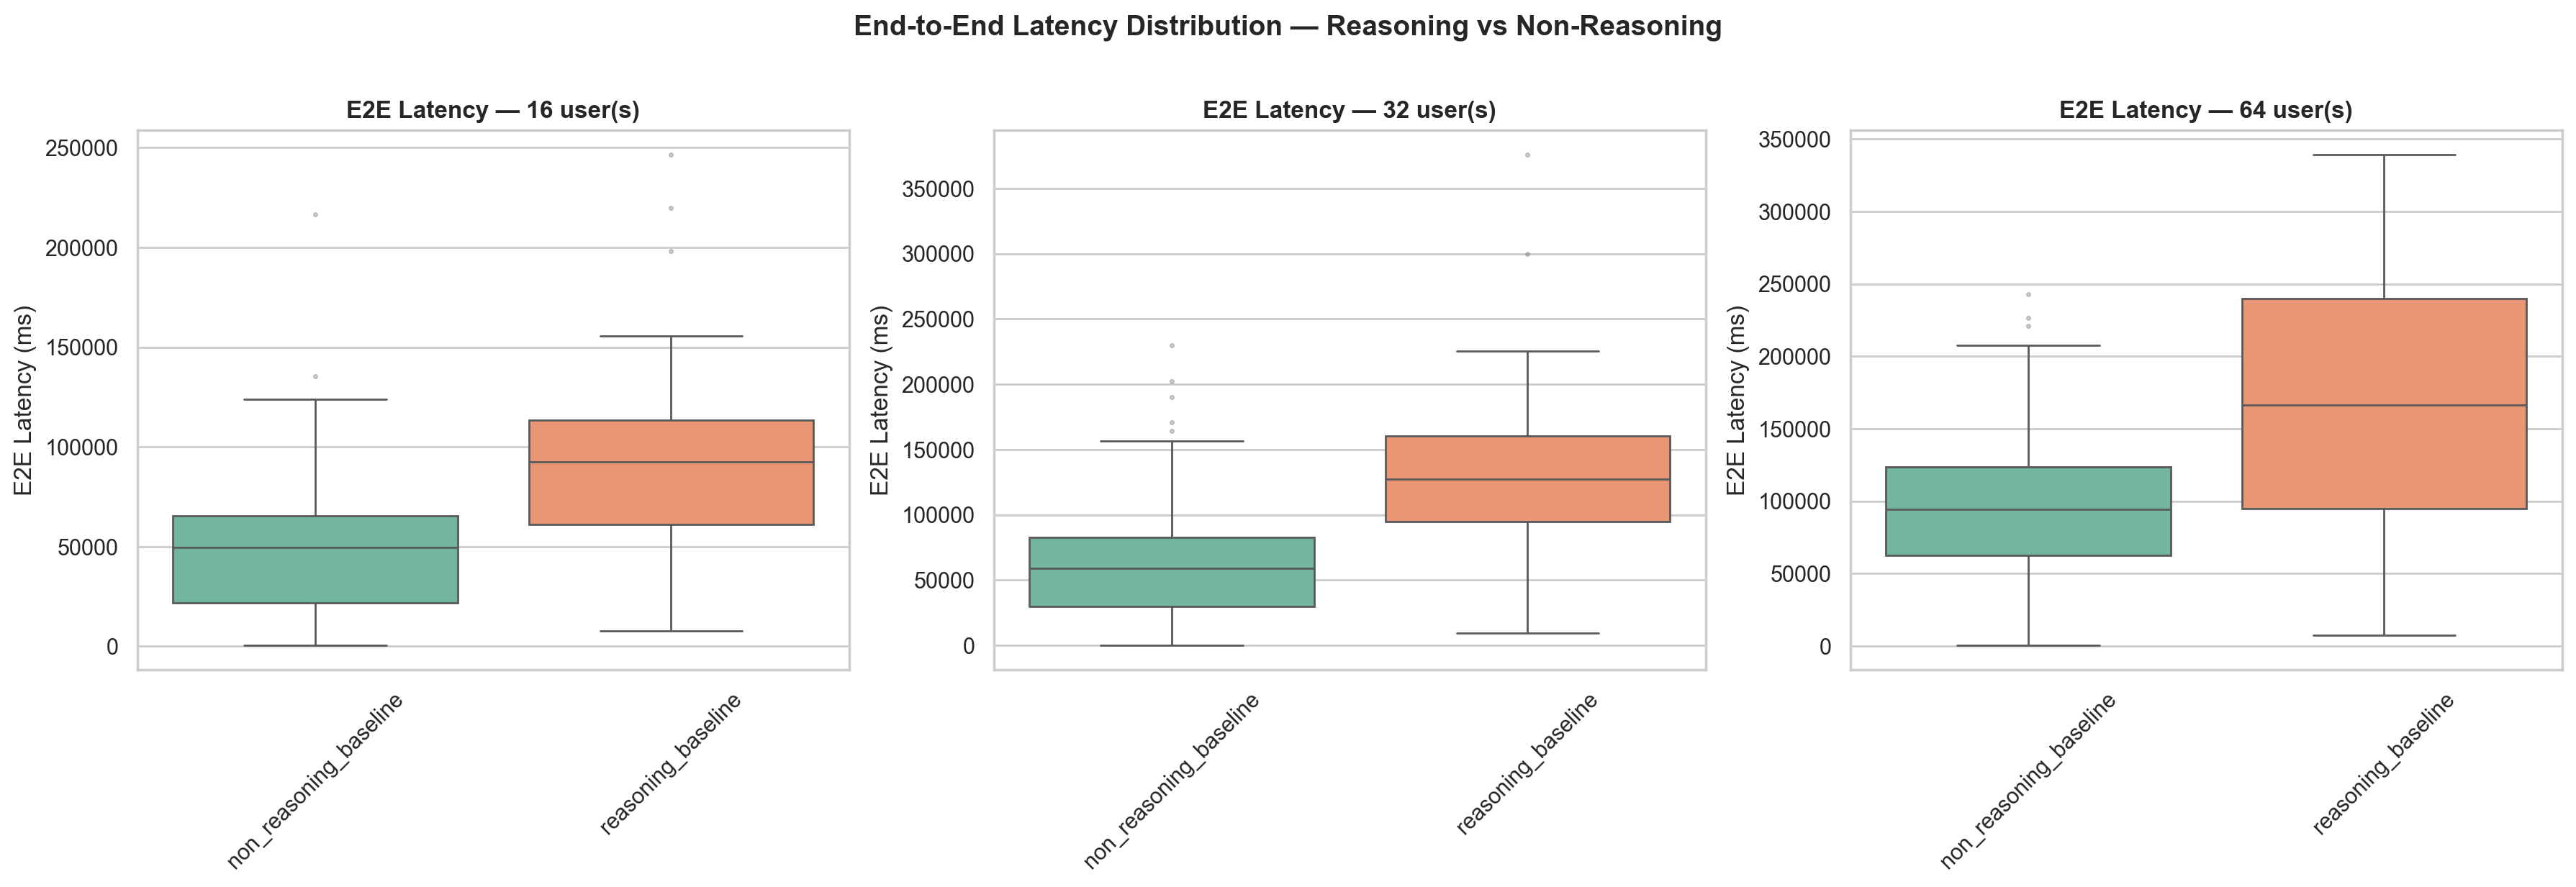
\includegraphics[width=0.9\textwidth]{../../benchmarking/results/run_20260404_181323/e2e_boxplot.png}
\caption{End-to-end latency distribution, Qwen3-8B reasoning vs.\ non-reasoning. The reasoning mode's chain-of-thought roughly doubles E2E latency.}
\label{fig:qwen3_e2e}
\end{figure}

\section{KV Cache Precision: Default vs.\ FP8 (Qwen3-8B)}

A second Qwen3-8B campaign (\texttt{run\_20260405\_005704}) compared the default (16-bit) KV cache against an FP8 KV cache, scaling concurrency up to 128 users.

\begin{table}[htbp]
\caption{Qwen3-8B KV cache: default (auto) vs.\ FP8, selected metrics.}
\centering
\begin{tabular}{|l|r|r|r|}
\hline
\textbf{Metric} & \textbf{Auto} & \textbf{FP8} & \textbf{Change} \\
\hline
TTFT P50 (u64) & 30{,}433 ms & 405 ms & $-99\%$ \\
TTFT P50 (u128) & 143{,}695 ms & 36{,}216 ms & $-75\%$ \\
E2E P50 (u128) & 188{,}400 ms & 124{,}353 ms & $-34\%$ \\
Throughput (u128) & 313 tok/s & 901 tok/s & $+188\%$ \\
Cost (u128) & \$1.40/M & \$0.49/M & $-65\%$ \\
Waiting reqs (u128) & 61.2 & 22.5 & $-63\%$ \\
\hline
\end{tabular}
\label{table:qwen3_kv}
\end{table}

The FP8 KV cache is the single most impactful Phase~1 lever at high concurrency. By halving the per-token KV footprint, it admits far more concurrent sequences before queuing: at u64 the default cache's TTFT collapses to 30~seconds while FP8 holds 405~ms, and at u128 FP8 sustains 901 tok/s---roughly $3\times$ the default's 313 tok/s---reaching the lowest cost of \$0.49/M tokens. Quality is unaffected (ARC 0.660, MMLU 0.797, GSM8K 0.879). This confirms the hypothesis that FP8 KV cache unlocks concurrency with negligible quality cost, and it became the default serving configuration for all subsequent work, including the Phase~2 Executor.

\begin{figure}[htbp]
\centering
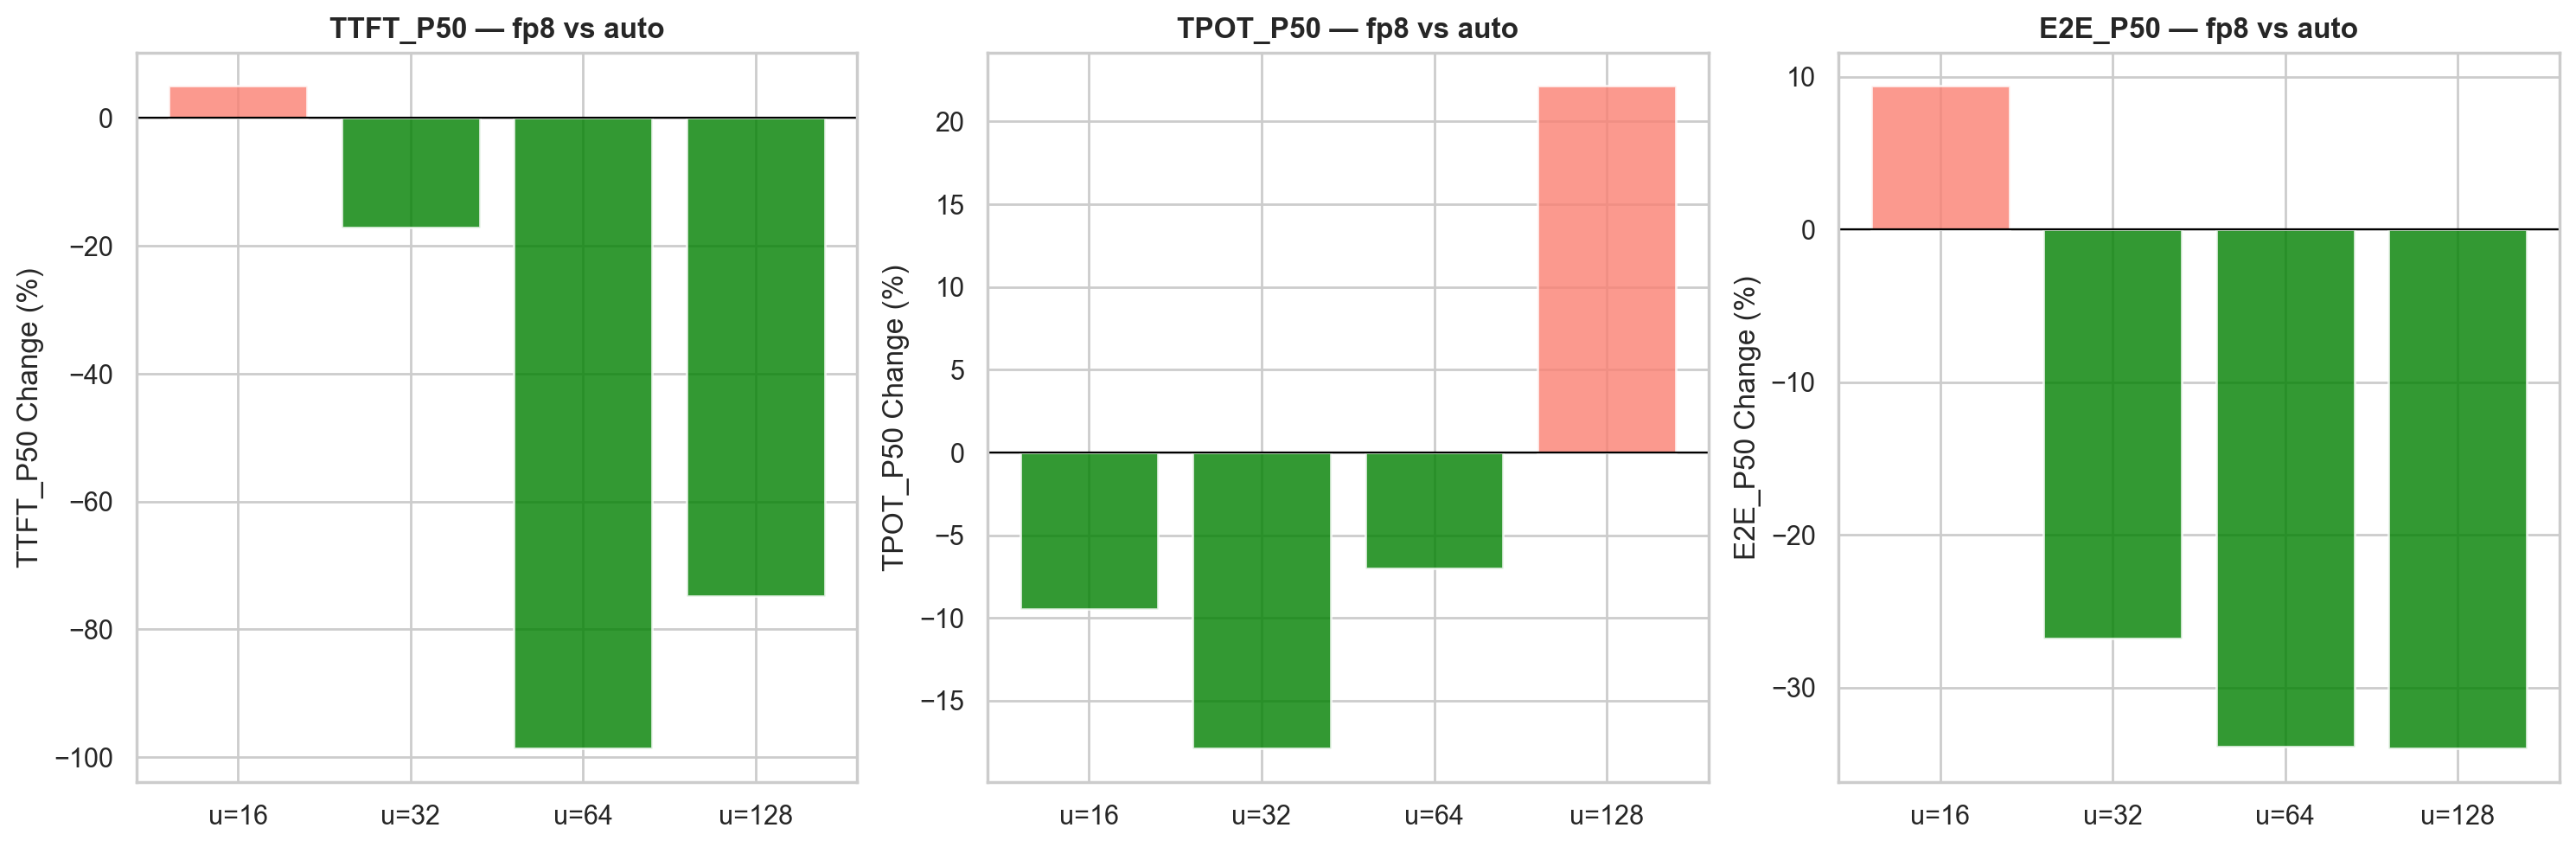
\includegraphics[width=0.92\textwidth]{../../benchmarking/results/run_20260405_005704/kv_cache_improvement.png}
\caption{FP8 KV cache improvement over the default cache (Qwen3-8B). Gains are largest at the highest concurrency, where the default cache saturates and queues.}
\label{fig:qwen3_kv_improvement}
\end{figure}

\begin{figure}[htbp]
\centering
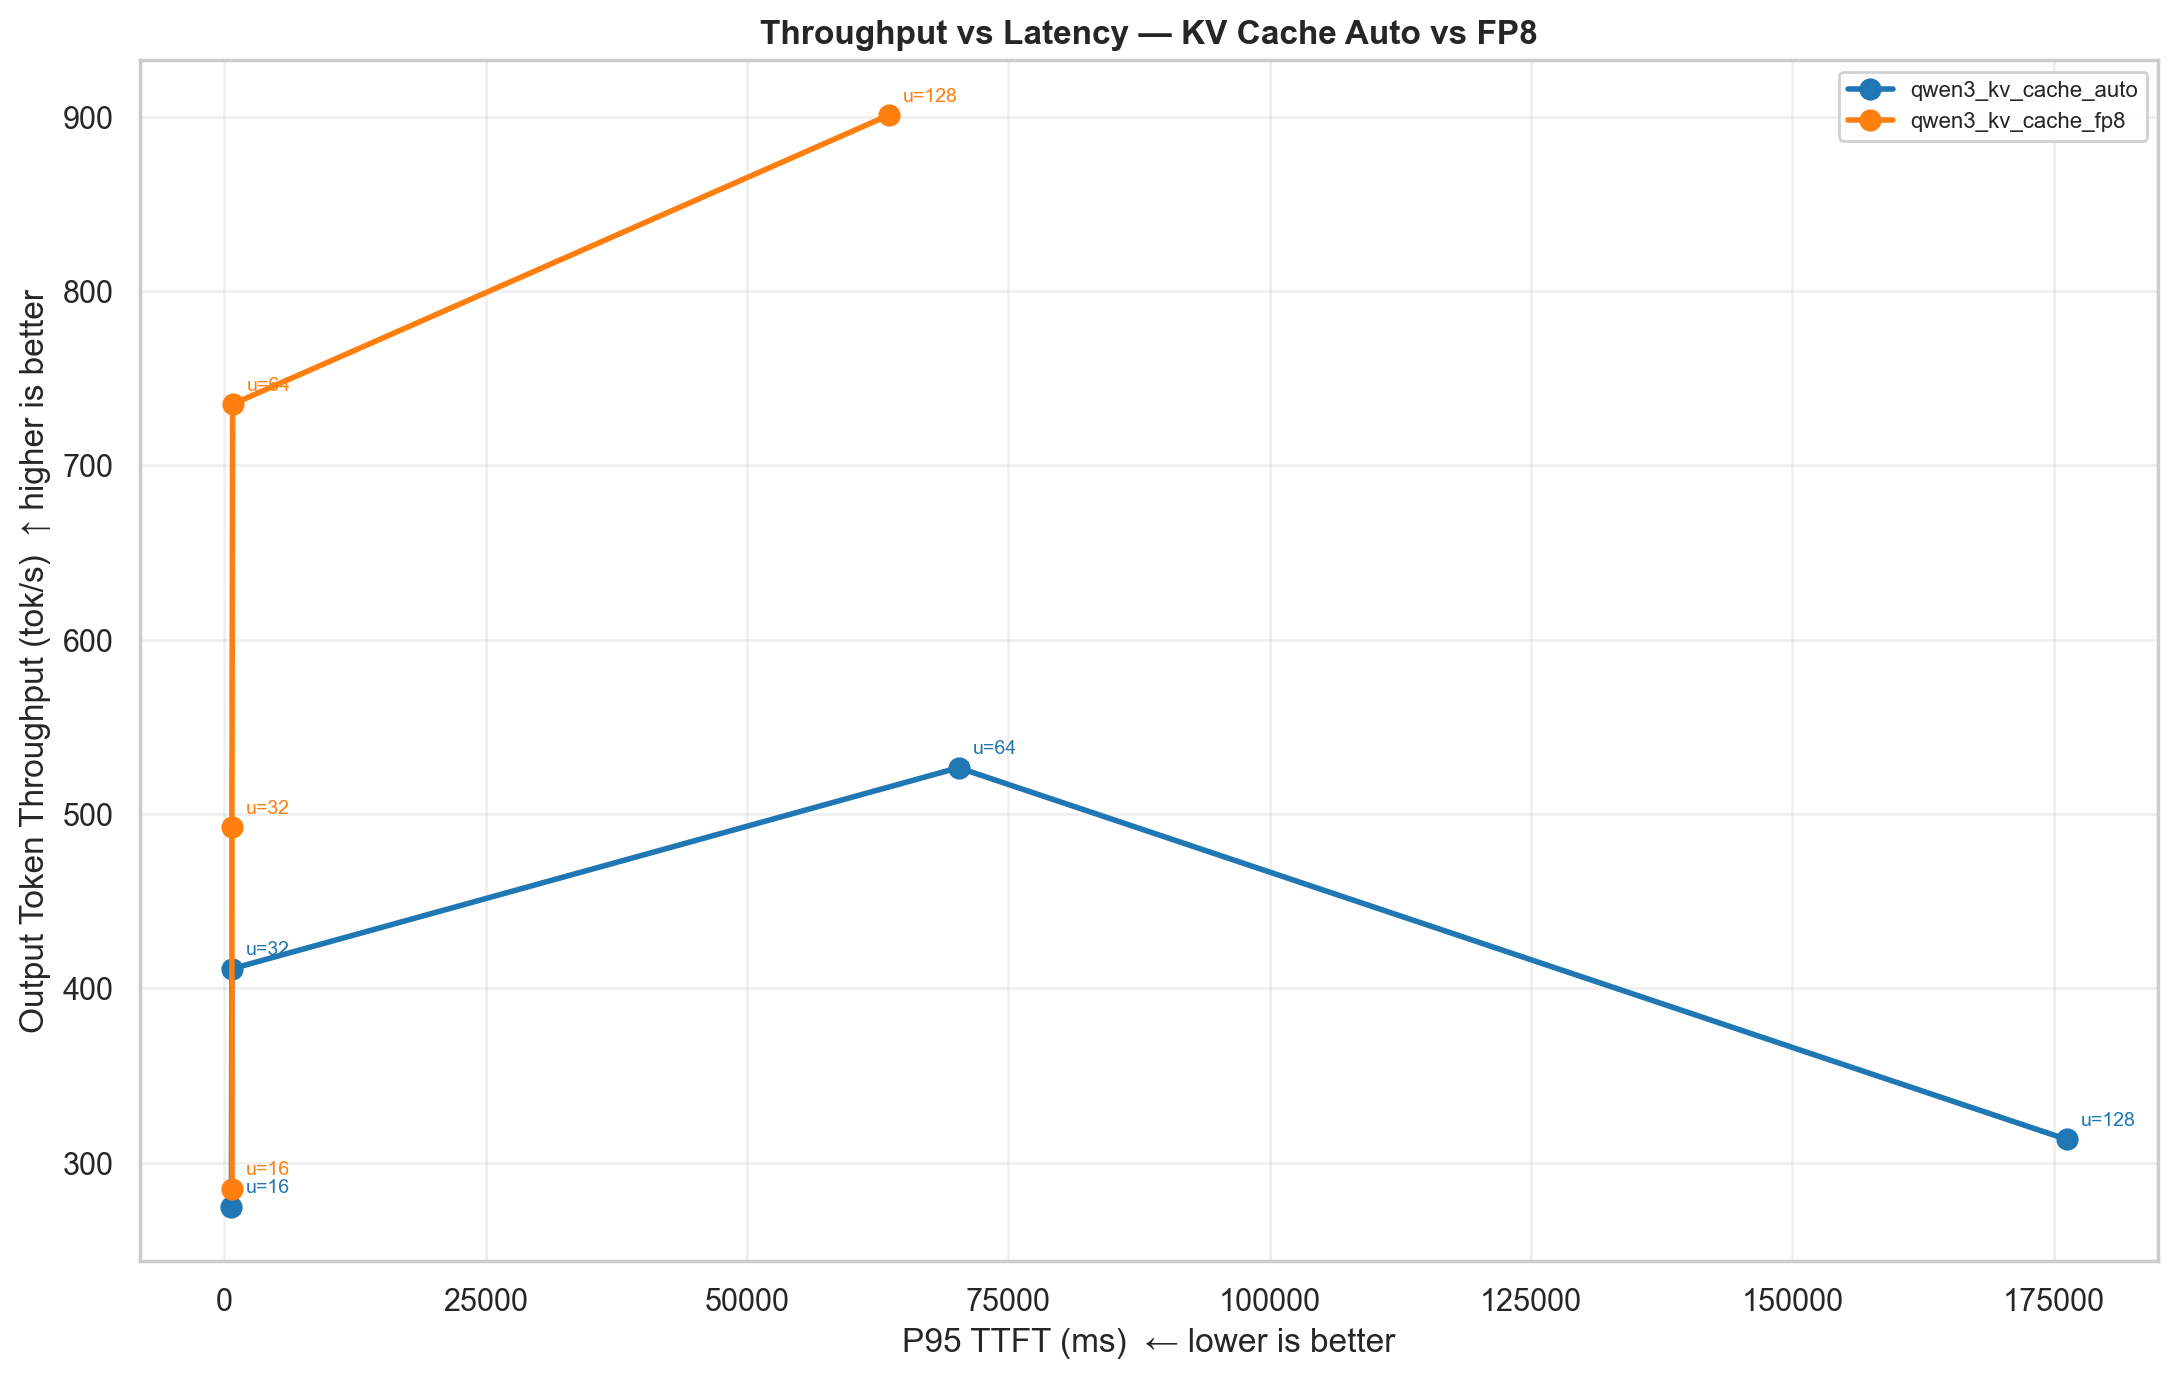
\includegraphics[width=0.92\textwidth]{../../benchmarking/results/run_20260405_005704/pareto_frontier.png}
\caption{Throughput vs.\ latency Pareto frontier, default vs.\ FP8 KV cache. FP8 dominates the frontier across concurrency levels.}
\label{fig:qwen3_kv_pareto}
\end{figure}

\section{TurboQuant KV-Cache Compression}

Having established FP8 as a strong baseline, the study tested whether more aggressive KV-cache compression (TurboQuant) could push further. Five presets were compared on Qwen3-8B (runs \texttt{run\_20260511\_234500} and \texttt{run\_20260512\_090311}) at 32/64/128 users: an FP8 baseline, \texttt{k8v4} (FP8 keys + 4-bit values), \texttt{4bit\_nc} (4-bit keys+values with norm correction), \texttt{k3v4\_nc} (3-bit keys + 4-bit values), and \texttt{3bit\_nc} (3-bit keys + 3-bit values).

\begin{table}[htbp]
\caption{TurboQuant vs.\ FP8 KV baseline (Qwen3-8B): throughput and cost.}
\centering
\begin{tabular}{|l|r|r|r|}
\hline
\textbf{Config} & \textbf{u128 tok/s} & \textbf{u128 \$/M} & \textbf{TPOT P50 vs.\ base} \\
\hline
fp8 (baseline) & \textbf{1{,}097} & \textbf{\$0.40} & --- \\
tq k8v4 & 292 & \$1.50 & $+28\%$ \\
tq 4bit\_nc & 575 & \$0.76 & $+59\%$ \\
tq k3v4\_nc & 760 & \$0.58 & $+88\%$ \\
tq 3bit\_nc & 392 & \$1.12 & $+106\%$ \\
\hline
\end{tabular}
\label{table:turboquant}
\end{table}

The results are clear and somewhat counter-intuitive: on the L4 with an 8B model, TurboQuant is \emph{not} worth it. Three findings dominate. First, the VRAM saving is tiny ($\sim$400~MiB out of 20.6~GiB) because the KV cache is only a small fraction of total VRAM---weights, activations, and allocator overhead dominate---so the compression does not free enough headroom to admit more concurrent requests (mean KV usage at u128 sits at 90--93\% for every variant including the baseline). Second, the dequantization compute lands directly on the decode path, inflating TPOT by 28--106\% and roughly doubling ITL on the 3-bit variants. Third, quality is essentially unchanged ($\pm$2.5~pp on ARC and GSM8K), so the compression buys no quality headroom either. The one niche advantage is TTFT under saturation: at u128 the smaller KV blocks let new requests admit 9--28\% faster, so a TurboQuant preset is defensible only when first-token responsiveness at extreme load matters more than throughput. Otherwise FP8 KV remains the best operating point at \$0.40/M tokens.

\begin{figure}[htbp]
\centering

\includegraphics[width=0.92\textwidth]{turboquant_pct_change_vs_baseline.png}
\caption{Percentage change of each TurboQuant preset relative to the FP8 KV baseline. Per-token decode (TPOT/ITL) regresses uniformly; throughput falls.}
\label{fig:turboquant_pct}
\end{figure}

\begin{figure}[htbp]
\centering

\includegraphics[width=0.9\textwidth]{turboquant_pareto_frontier.png}
\caption{Throughput vs.\ P95 TTFT Pareto frontier for TurboQuant presets. The FP8 baseline dominates on throughput; TurboQuant only wins on admit-time TTFT under saturation.}
\label{fig:turboquant_pareto}
\end{figure}

\section{Model Comparison: Gemma~4 vs.\ Qwen3-8B}

Finally, the serving study compared two model families at matched FP8 KV configuration (run \texttt{run\_20260416\_010036} vs.\ the Qwen3 FP8 run): Google's Gemma~4 E4B against Qwen3-8B.

\begin{table}[htbp]
\caption{Gemma~4 E4B vs.\ Qwen3-8B (FP8 KV), selected metrics.}
\centering
\begin{tabular}{|l|r|r|}
\hline
\textbf{Metric} & \textbf{Gemma~4 E4B} & \textbf{Qwen3-8B} \\
\hline
TTFT P50 (u128) & 525 ms & 36{,}216 ms \\
TPOT P50 (u128) & 102.0 ms/tok & 124.7 ms/tok \\
Throughput (u128) & 1{,}880 tok/s & \textbf{3{,}599 tok/s} \\
Cost (u128) & \$0.23/M & \textbf{\$0.12/M} \\
ARC-Challenge & 0.31 & \textbf{0.65} \\
GSM8K & 0.70 & \textbf{0.88} \\
\hline
\end{tabular}
\label{table:gemma_qwen}
\end{table}

The two models occupy different niches. Gemma~4 E4B is extraordinarily resilient to queueing---at u128 it holds a 525~ms TTFT where Qwen3 spikes to an unusable 36.2~seconds---and has slightly better TPOT at every level. But Qwen3-8B delivers far higher peak throughput (3{,}599 vs.\ 1{,}880 tok/s, making it nearly twice as cost-effective at \$0.12/M) and decisively higher quality (ARC 65\% vs.\ 31\%, GSM8K 88\% vs.\ 70\%). For a throughput- and quality-oriented serving backend, Qwen3-8B is preferred; Gemma~4's stability advantage is most valuable for latency-critical, interactive workloads.

\begin{figure}[htbp]
\centering
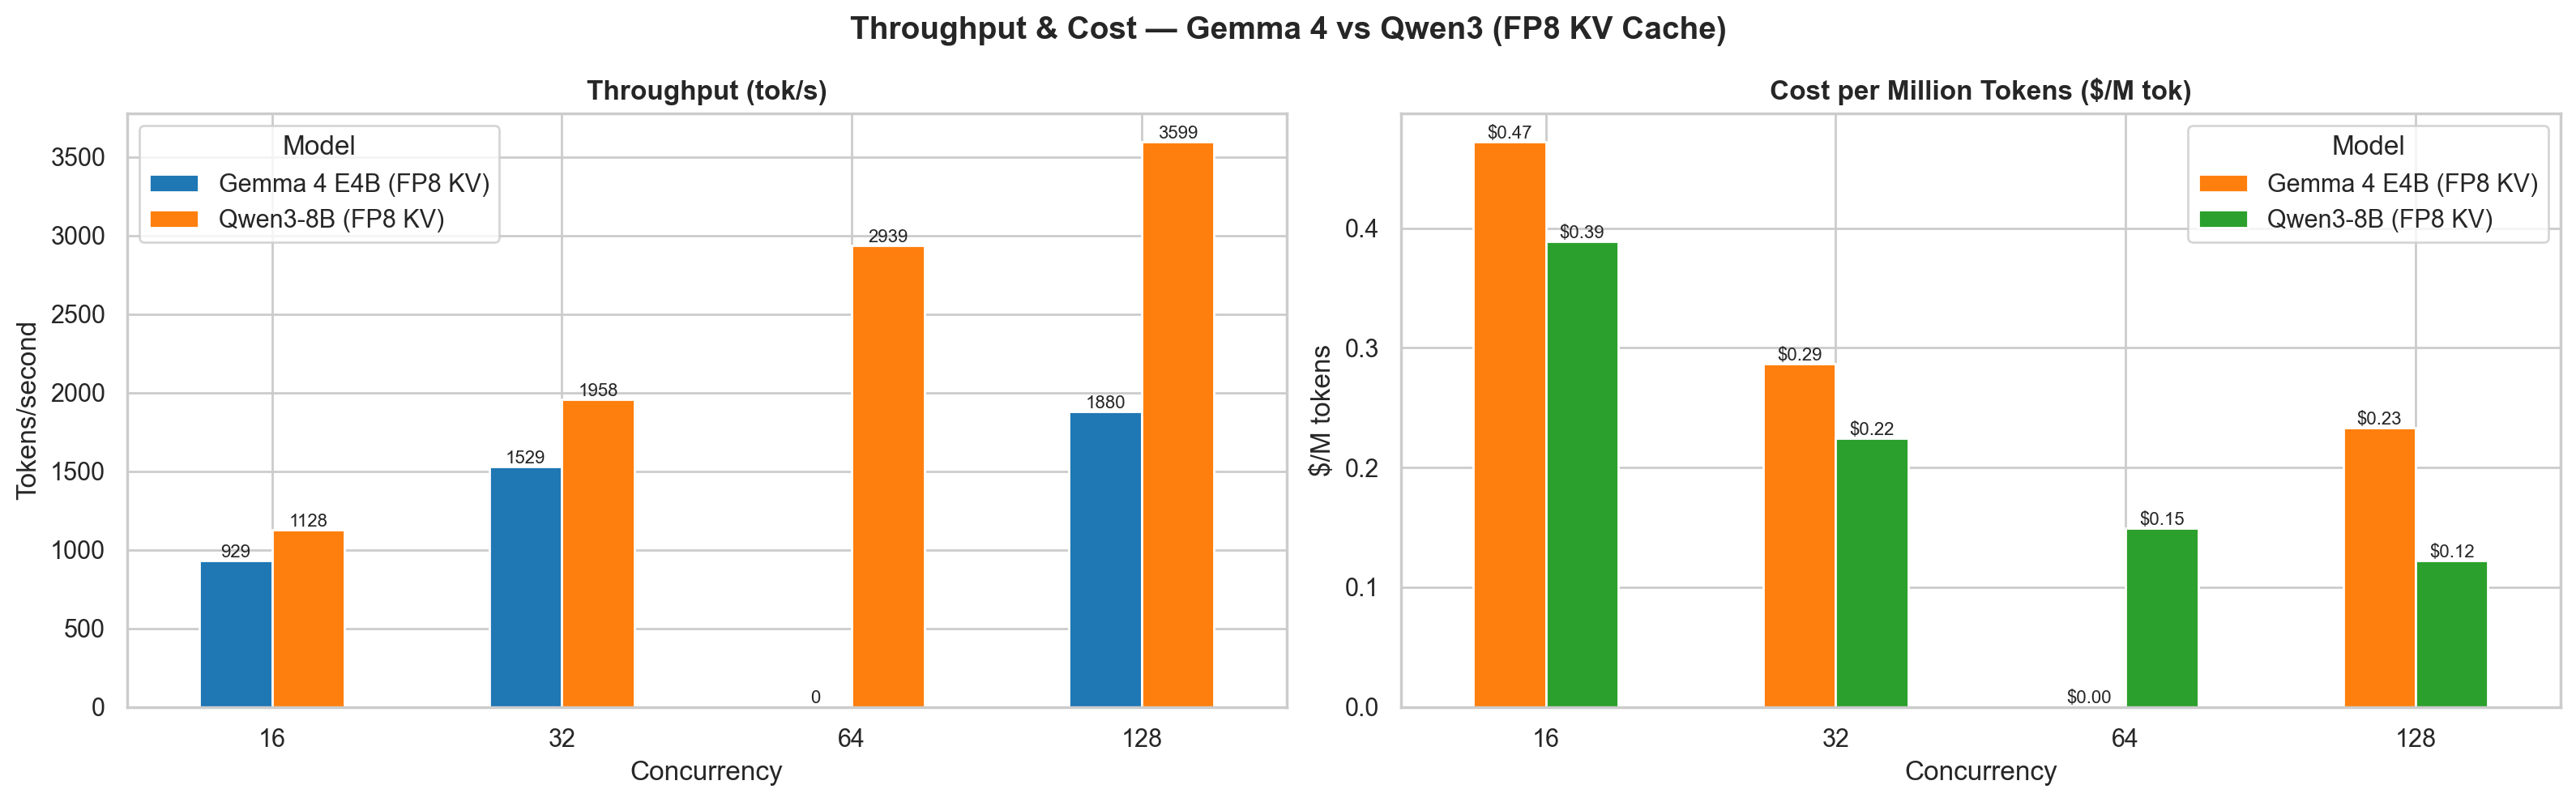
\includegraphics[width=0.92\textwidth]{../../benchmarking/results/gemma4_vs_qwen3_comparison/throughput_cost.png}
\caption{Throughput and cost, Gemma~4 E4B vs.\ Qwen3-8B (FP8 KV). Qwen3 reaches far higher peak throughput and lower cost per token.}
\label{fig:gemma_qwen_throughput}
\end{figure}

\begin{figure}[htbp]
\centering
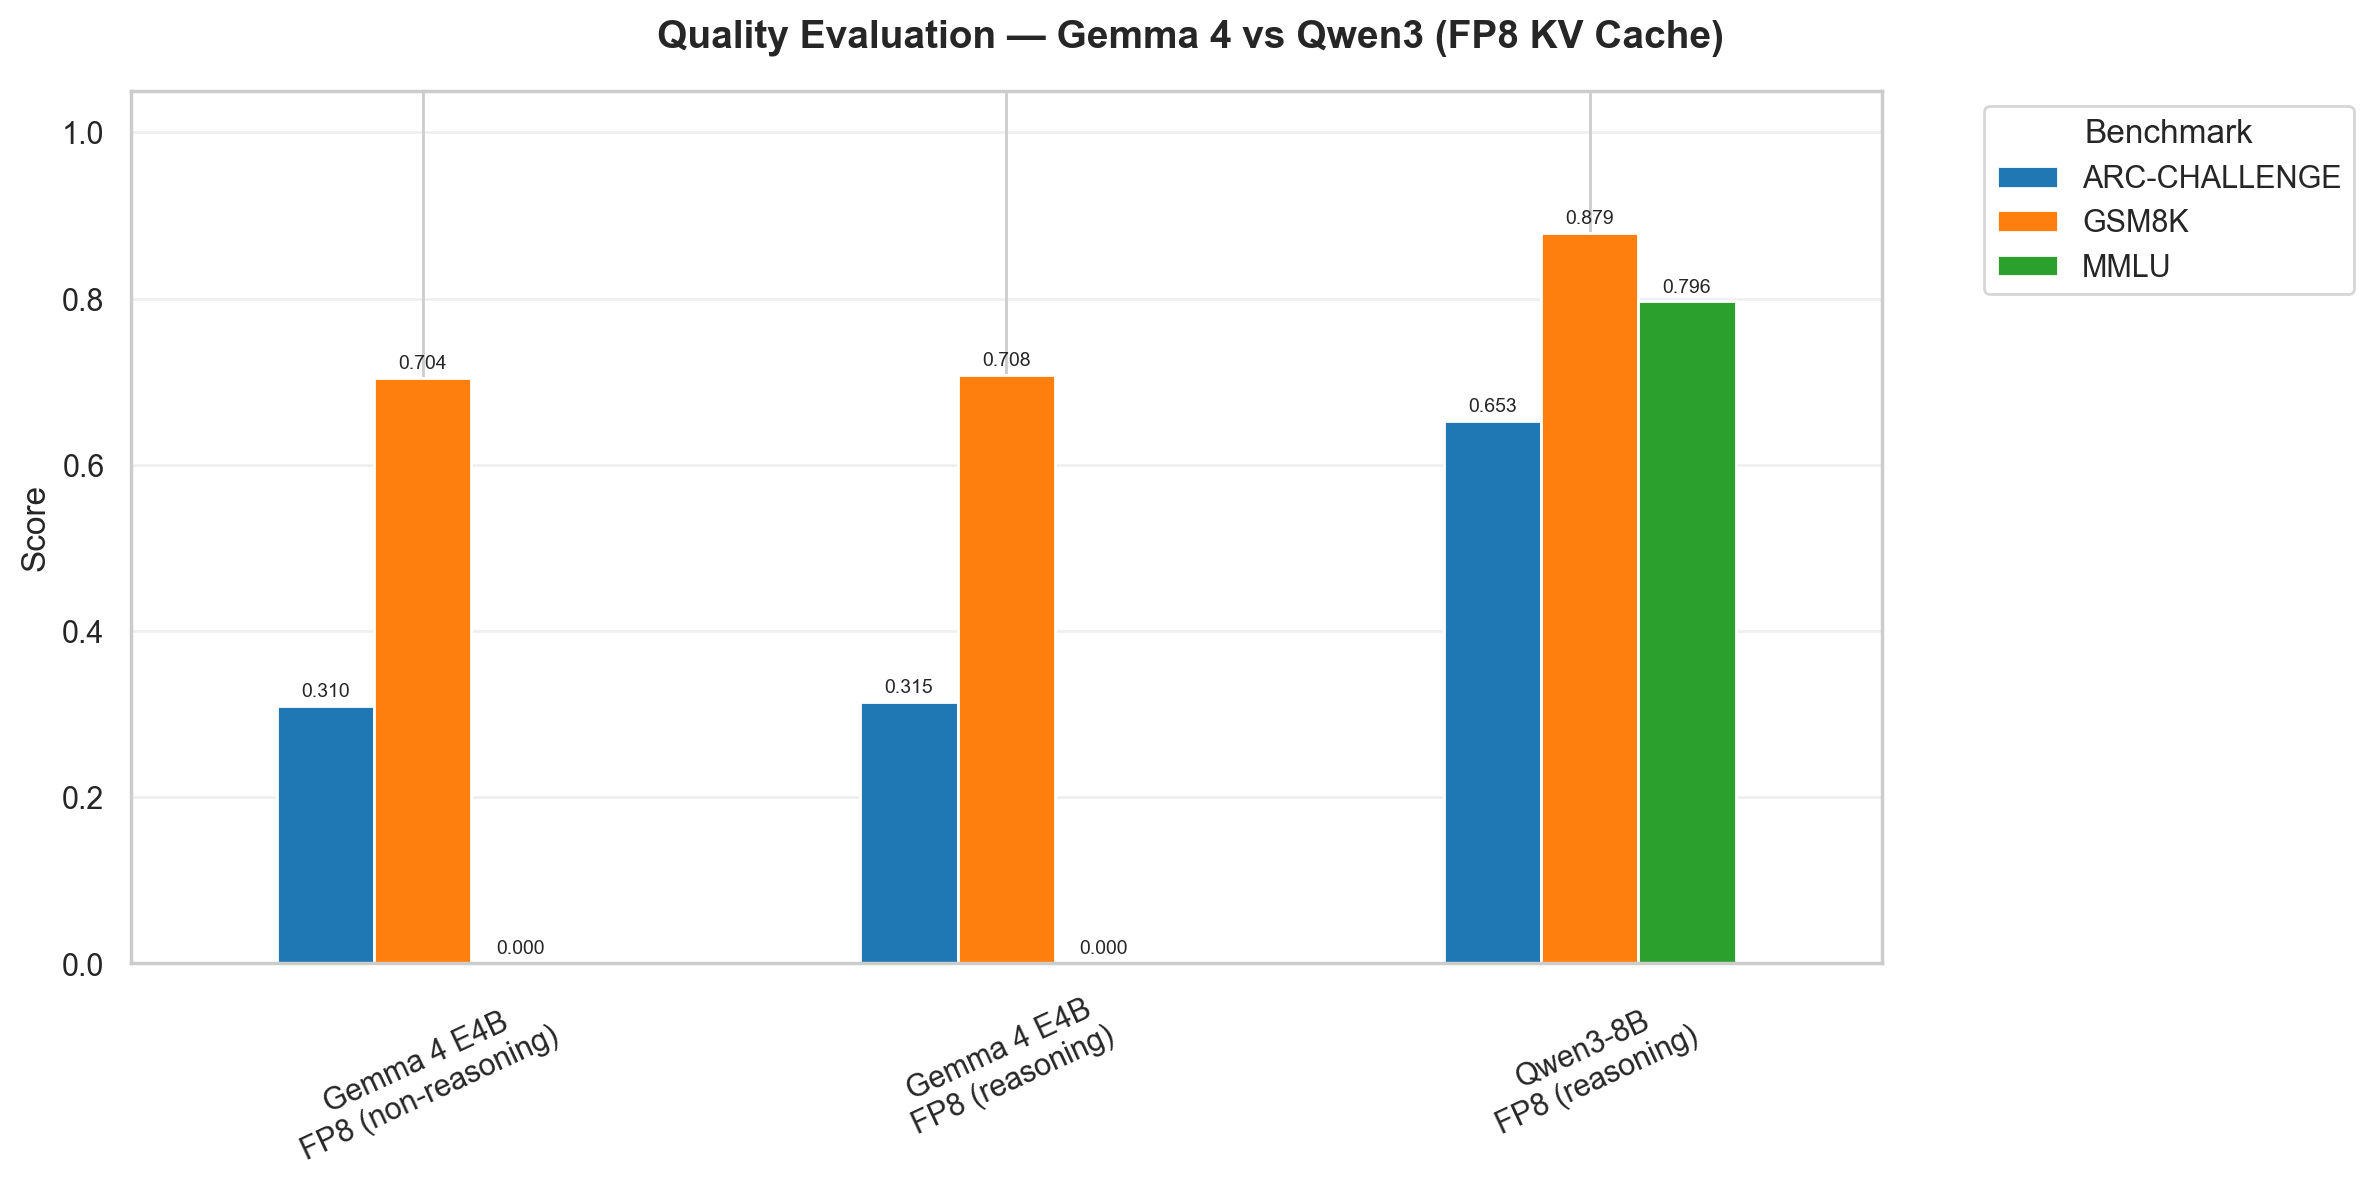
\includegraphics[width=0.9\textwidth]{../../benchmarking/results/gemma4_vs_qwen3_comparison/quality_comparison.png}
\caption{Quality comparison, Gemma~4 E4B vs.\ Qwen3-8B. Qwen3 substantially outscores Gemma~4 on ARC-Challenge and GSM8K.}
\label{fig:gemma_qwen_quality}
\end{figure}

\section*{Part II --- Phase 2: Asymmetric Agent on GAIA}
\addcontentsline{toc}{section}{Part II --- Phase 2: Asymmetric Agent on GAIA}

Phase~2 evaluates five agent configurations on the GAIA Level~1 validation set (53 multi-step questions requiring web search, file handling, and code execution). The Executor, where self-hosted, is the AWQ 4-bit Gemma~4 26B served by the FP8-optimized vLLM stack from Phase~1; the Planner, where commercial, is Gemini~3 Flash. Each configuration is measured on accuracy, mean task duration, and cost per question.

\begin{table}[htbp]
\caption{GAIA Level~1 results across agent configurations. Cost is the cost-adjusted figure (self-hosted Executor tokens imputed a price).}
\centering
\begin{tabular}{|p{4.6cm}|r|r|r|}
\hline
\textbf{Configuration} & \textbf{Accuracy} & \textbf{Cost/Q} & \textbf{Duration} \\
\hline
Large-Planner-Executor (Gemini + Gemini) & \textbf{84.9\%} & \$0.1207 & 356 s \\
Planner-Only (Gemini direct) & 73.6\% & \$0.0363 & 319 s \\
\textbf{Planner-Executor (Gemini + Gemma~4)} & \textbf{67.9\%} & \textbf{\$0.0110} & 278 s \\
Single-Agent (Gemma~4 direct) & 50.9\% & \$0.0050 & 106 s \\
Small-Planner-Executor (Gemma~4 + Gemma~4) & 39.6\% & \$0.0021 & 651 s \\
\hline
\end{tabular}
\label{table:gaia}
\end{table}

The headline result is the \textbf{hybrid Planner--Executor} configuration (commercial Gemini Planner + self-hosted Gemma~4 Executor). It achieves 67.9\% accuracy---about 80\% of the all-commercial ceiling of 84.9\%---while costing \$0.0110 per question, roughly \textbf{one-tenth} of the all-commercial baseline's \$0.1207. In other words, offloading the high-volume execution work to the self-hosted model preserves four-fifths of the quality at one-tenth of the cost, placing the hybrid on the Pareto frontier of the accuracy-versus-cost space.

The other configurations frame this result. The all-commercial \texttt{Large-Planner-Executor} sets the quality ceiling but is by far the most expensive. \texttt{Planner-Only}, calling Gemini directly without a separate executor, is cheaper but loses 11~pp of accuracy---confirming that an explicit plan-then-execute decomposition helps. At the low end, the fully self-hosted \texttt{Single-Agent} reaches a respectable 50.9\% at near-zero marginal cost, while the fully self-hosted \texttt{Small-Planner-Executor} actually \emph{regresses} to 39.6\% and the longest duration (651~s): a weak planner produces verbose, sometimes misleading plans that the same weak model then struggles to execute, so the two-model overhead is not repaid. The clear lesson is that planning quality is what must be bought from the frontier model; execution can be safely and cheaply self-hosted.

\begin{figure}[htbp]
\centering
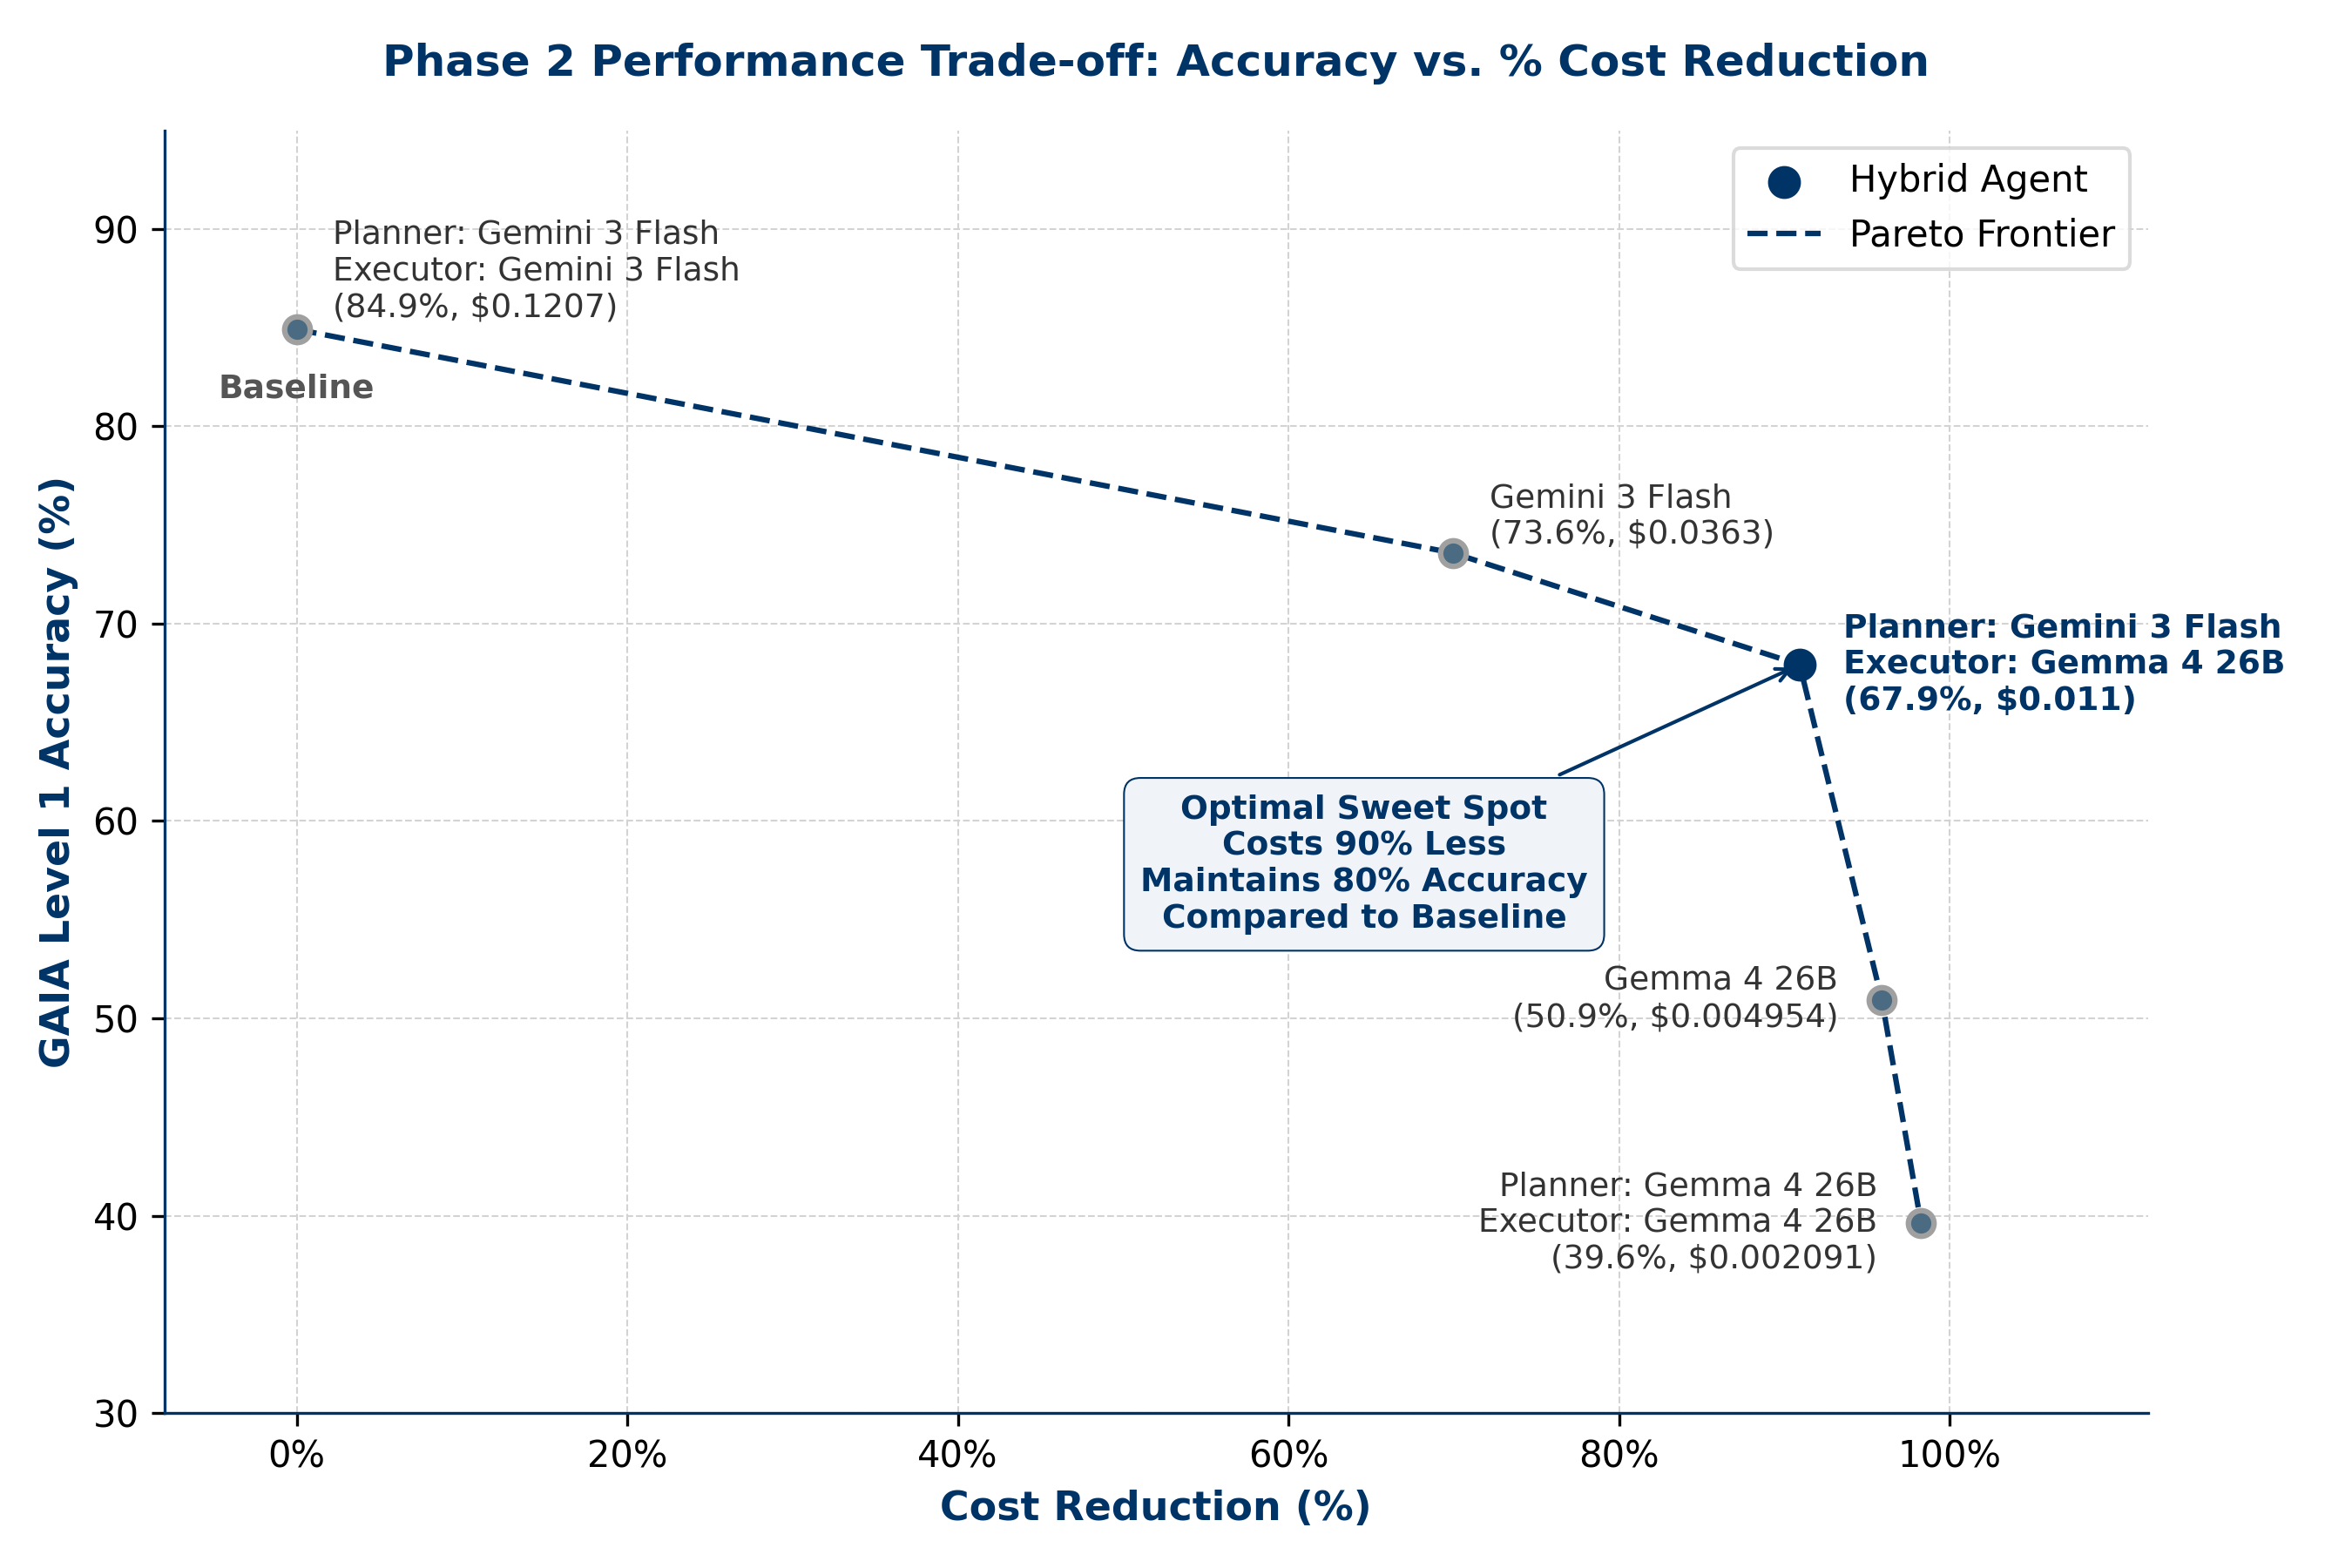
\includegraphics[width=0.95\textwidth]{../../evaluation/agent-results/phase2_pareto_cost_adjusted_percentage.png}
\caption{Phase~2 accuracy vs.\ cost-reduction trade-off on GAIA Level~1. The hybrid Planner--Executor is the Pareto-optimal ``sweet spot'': $\sim$90\% cheaper than the all-commercial baseline while retaining $\sim$80\% of its accuracy.}
\label{fig:phase2_pareto}
\end{figure}

To validate that the self-hosted Executor can sustain agentic traffic, the Phase~1 Locust harness was extended with an agent workload (\texttt{locustfile\_agent.py}, \texttt{agent\_load\_test.json}) that drives the agent API end-to-end through the vLLM Executor. The serving layer handled this concurrent agentic load using the same FP8 KV configuration validated in Phase~1, closing the loop between the two phases: the optimization measured in Phase~1 is exactly what makes the Phase~2 Executor economically viable.

% ============================================================
\chapter{CONCLUSION}
% ============================================================

\section{Summary of Findings}

This project produced the following primary findings from a two-phase study: a systematic serving-optimization benchmarking campaign for vLLM on NVIDIA L4 GPUs (Phase~1), and a GAIA evaluation of a hybrid Planner--Executor agent built on the optimized serving layer (Phase~2):

\textbf{Finding 1: FP8 quantization is the clear recommendation for production LLM serving.} It reduces TTFT P50 by 28--30\%, TPOT P50 by 3--35\%, and E2E P50 by 6--35\% relative to FP16, while causing less than 2.4\% quality degradation on ARC-Challenge, MMLU, and GSM8K. The cost per million output tokens drops from \$1.67 to \$1.46 at 16 users and from \$0.68 to \$0.47 at 64 users.

\textbf{Finding 2: BitsAndBytes (INT4) quantization is counterproductive on the L4 GPU.} It doubles TPOT (to 138 ms/tok), increases E2E latency by 181\%, and increases cost per million tokens by 93\% relative to FP16. This is because the L4 lacks native INT4 compute, and the BitsAndBytes dequantization overhead exceeds the memory bandwidth savings.

\textbf{Finding 3: Higher concurrency is the dominant cost-reduction lever.} Moving from 16 to 64 concurrent users reduces cost per million tokens from \$1.67 to \$0.68 for the FP16 baseline (a 2.5$\times$ reduction)---larger than any single parameter change. FP8 at u=64 achieves \$0.47/M tokens, 6.85$\times$ cheaper than BitsAndBytes at u=16.

\textbf{Finding 4: Reasoning models are significantly more expensive to serve.} DeepSeek-R1's E2E P50 (71{,}382 ms) is 70\% higher than Qwen2.5's (41{,}955 ms) at identical concurrency and precision, purely because of chain-of-thought output tokens. Applications that do not require step-by-step reasoning should prefer non-reasoning models.

\textbf{Finding 5: TTFT is insensitive to input prompt length within the 4096-token window.} Across all I/O profiles tested (short inputs of $\approx$15 tokens to long inputs of $\approx$140 tokens), TTFT P50 stays in the 185--195 ms range at 16 users. The L4's prefill throughput does not become a bottleneck for prompt lengths below several thousand tokens.

\textbf{Finding 6: E2E latency is driven by output length, not input length.} Short-input prompts finish 3.4$\times$ faster than long-input prompts, but this is because longer prompts elicit longer reasoning chains, not because of prefill overhead.

\textbf{Finding 7: Prefix caching provides up to 55\% TTFT reduction for shared-prefix workloads.} At 8 concurrent users with a shared system prompt, enabling prefix caching reduces TTFT P50 by 53.7--55.7\%. The benefit is negligible at u=1 (cold cache) and grows with concurrency. This makes prefix caching essential for production chatbot deployments where a system prompt is repeated in every request.

\textbf{Finding 8: KV cache is not a bottleneck for 7B models on 24 GB GPUs.} KV cache utilization peaked at 5.4\% across all tested configurations. Parameters like \texttt{gpu-memory-utilization} have no measurable effect in this regime. This would change significantly with larger models or longer context windows.

\textbf{Finding 9: An FP8 KV cache is the most impactful high-concurrency lever.} On Qwen3-8B, switching from the default cache to an FP8 KV cache cut TTFT at u64 from 30~seconds to 405~ms, tripled throughput at u128 (313 $\to$ 901 tok/s), and lowered cost by 65\% (\$1.40 $\to$ \$0.49/M)---all with no measurable quality loss. FP8 KV became the default configuration for the rest of the project.

\textbf{Finding 10: Aggressive KV-cache compression (TurboQuant) does not pay off on the L4.} Across five presets up to 3-bit keys+values, VRAM savings were negligible ($\sim$400~MiB of 20.6~GiB), throughput fell at every concurrency level, and TPOT regressed by 28--106\%, while quality stayed within $\pm$2.5~pp. The only advantage was faster first-token admit-time under saturation. The technique would likely help on larger models or hardware with cheaper dequant paths, but FP8 KV remains the best operating point here.

\textbf{Finding 11: Model choice is a real trade-off.} Qwen3-8B offers far higher peak throughput (3{,}599 tok/s, \$0.12/M) and decisively higher quality than Gemma~4 E4B, while Gemma~4 is dramatically more stable under extreme concurrency (525~ms TTFT at u128 vs.\ Qwen3's 36~s). The right choice depends on whether the workload prioritizes throughput and quality or tail-latency stability.

\textbf{Finding 12: The hybrid Planner--Executor agent is the Pareto-optimal architecture.} On GAIA Level~1, pairing a commercial Planner (Gemini~3 Flash) with a self-hosted Gemma~4 Executor achieved 67.9\% accuracy---$\sim$80\% of the all-commercial ceiling (84.9\%)---at \$0.0110 per question, about one-tenth of the all-commercial cost. Planning quality must be bought from the frontier model; execution can be cheaply self-hosted. A fully self-hosted two-model agent (\texttt{small-planner-executor}) regressed to 39.6\%, showing that a weak planner is worse than none.

\section{Practical Recommendations}

\begin{table}[h!]
\caption{Configuration recommendations for different goals.}
\centering
\begin{tabular}{|p{4cm}|p{9cm}|}
\hline
\textbf{Goal} & \textbf{Recommendation} \\
\hline
Lowest latency & FP8 quantization + high concurrency (u=64+) \\
\hline
Lowest cost per token & FP8 + u=64 (\$0.47/M tokens on L4) \\
\hline
Best quality & FP16 baseline (marginal gain over FP8, max 2.4\%) \\
\hline
Best quality/latency/cost balance & FP8 --- Pareto-optimal across all benchmarks \\
\hline
Chatbot with system prompts & Enable prefix caching (up to 55\% TTFT reduction) \\
\hline
High-concurrency serving & Enable FP8 KV cache (up to 3$\times$ throughput, no quality loss) \\
\hline
Tail-latency-critical workload & Gemma~4 (sub-600~ms TTFT even at u=128) \\
\hline
Cost-efficient agent & Hybrid Planner--Executor (commercial Planner + self-hosted Executor) \\
\hline
Avoid & BitsAndBytes; TurboQuant on L4; a fully self-hosted two-model agent \\
\hline
\end{tabular}
\label{table:recommendations}
\end{table}

\section{Limitations}

\begin{enumerate}
    \item All experiments used a single GPU (L4). Results may differ on A100, H100, or multi-GPU setups.
    \item The maximum concurrency tested was 64 users. At higher concurrency, KV cache exhaustion and queuing effects not observed here may emerge.
    \item Test duration was 90 seconds per sub-test. Longer tests would better characterize steady-state behavior and thermal throttling effects.
    \item Requests are single-turn; multi-turn conversations create different KV cache reuse patterns.
    \item The custom prompt dataset (37 prompts) is small and may not fully represent production workload diversity.
    \item BitsAndBytes testing was limited to u=16; u=64 data was not available due to infrastructure issues.
    \item The Phase~2 agent was evaluated only on GAIA Level~1 (53 questions); Levels~2 and~3 and larger sample sizes would tighten the accuracy estimates and stress harder multi-hop reasoning.
    \item Phase~2 cost figures depend on an imputed price for self-hosted tokens derived from Phase~1 throughput; the absolute cost ratio would shift with a different GPU rate or utilization assumption.
\end{enumerate}

\section{Future Work}

\begin{enumerate}
    \item \textbf{Dynamic task routing}: Implement a lightweight router that sends simple queries directly to the self-hosted Executor, bypassing the Planner API entirely to further reduce cost while reserving the commercial Planner for genuinely complex tasks.
    \item \textbf{Executor fine-tuning}: Distill the Planner's reasoning patterns and tool-use traces into the local Executor (Gemma~4) to close the accuracy gap between the hybrid and the all-commercial agent.
    \item \textbf{Hardware scaling}: Re-run the aggressive KV-cache compression (TurboQuant) and FP8 experiments on newer GPUs (H100/H200), where native FP8/INT4 acceleration should eliminate the dequantization compute bottleneck observed on the L4.
    \item Extend the experiment matrix to speculative decoding, which can further reduce TPOT by using a small draft model to propose tokens verified by the main model in batch.
    \item Evaluate multi-GPU tensor parallelism (TP=2, TP=4) and longer context workloads (8K--128K tokens), where KV cache management becomes the dominant bottleneck and KV compression may finally pay off.
    \item Broaden the agent evaluation to GAIA Levels~2 and~3 and additional agent benchmarks, and integrate the serving pipeline with the MLCommons MLPerf Inference suite for standardized cross-system comparison.
\end{enumerate}

\bibliographystyle{plain}
\bibliography{references}

% ============================================================
\appendix

\chapter{vLLM PARAMETER REFERENCE}
% ============================================================

\section{Install-Time Parameters}

vLLM compiles custom CUDA kernels at install time. The hardware platform (NVIDIA CUDA, AMD ROCm, Intel XPU, CPU-only) and the target GPU compute capabilities (\texttt{TORCH\_CUDA\_ARCH\_LIST}) must be specified at build time. Pre-built pip wheels include support for all common NVIDIA architectures (T4=7.5, A100=8.0, L4=8.9, H100=9.0). Using the Docker image \texttt{vllm/vllm-openai:latest} avoids CUDA version mismatch issues.

\section{Key Runtime Parameters (\texttt{vllm serve})}

\begin{longtable}{|p{5cm}|p{2.5cm}|p{6cm}|}
\caption{Key vLLM runtime parameters used in this project.} \\
\hline
\textbf{Parameter} & \textbf{Default} & \textbf{Description} \\
\hline
\endfirsthead
\hline
\textbf{Parameter} & \textbf{Default} & \textbf{Description} \\
\hline
\endhead
\texttt{--model} & ---  & HuggingFace model ID or local path \\
\hline
\texttt{--dtype} & auto & Weight precision: half, bfloat16, float16 \\
\hline
\texttt{--max-model-len} & from config & Maximum context length in tokens \\
\hline
\texttt{--quantization} & None & Quantization: fp8, bitsandbytes, awq, gptq \\
\hline
\texttt{--gpu-memory-utilization} & 0.9 & Fraction of GPU VRAM for KV cache \\
\hline
\texttt{--max-num-seqs} & 128 & Max concurrent sequences per batch \\
\hline
\texttt{--enable-chunked-prefill} & auto & Split long prefills to reduce head-of-line blocking \\
\hline
\texttt{--enable-prefix-caching} & auto & Reuse KV blocks for shared prompt prefixes \\
\hline
\texttt{--tensor-parallel-size} & 1 & Number of GPUs for tensor parallelism \\
\hline
\texttt{--port} & 8000 & HTTP server port \\
\hline
\end{longtable}

\chapter{EXPERIMENT CONFIGURATIONS}

\section{Server Tuning Experiments (Pilot)}

\begin{table}[h!]
\caption{Server tuning experiment configurations tested in the pilot study.}
\centering
\begin{tabular}{|l|l|l|}
\hline
\textbf{Name} & \textbf{Changed Parameter} & \textbf{Concurrency} \\
\hline
baseline & --- (defaults) & 1, 4, 8 \\
max\_seqs\_8 & \texttt{--max-num-seqs 8} & 1, 4, 8 \\
max\_seqs\_32 & \texttt{--max-num-seqs 32} & 1, 8, 32 \\
gpu\_mem\_80 & \texttt{--gpu-memory-utilization 0.80} & 1, 4, 8 \\
gpu\_mem\_95 & \texttt{--gpu-memory-utilization 0.95} & 1, 4, 8, 16 \\
chunked\_prefill & \texttt{--enable-chunked-prefill} & 1, 4, 8 \\
prefix\_caching & \texttt{--enable-prefix-caching} & 1, 4, 8 \\
chunked\_prefill + prefix\_caching & both & 1, 4, 8, 16 \\
\hline
\end{tabular}
\end{table}

\section{Quantization Experiments}

\begin{table}[h!]
\caption{Quantization experiment configurations.}
\centering
\begin{tabular}{|l|l|l|}
\hline
\textbf{Name} & \textbf{Model} & \textbf{vLLM Args} \\
\hline
baseline & DeepSeek-R1 & FP16 (default) \\
fp8\_quantization & DeepSeek-R1 & \texttt{--quantization fp8} \\
bitsandbytes\_quantization & DeepSeek-R1 & \texttt{--quantization bitsandbytes} \\
non\_reasoning\_baseline & Qwen2.5-7B & non-reasoning config \\
non\_reasoning\_fp8 & Qwen2.5-7B & \texttt{--quantization fp8} \\
non\_reasoning\_bitsandbytes & Qwen2.5-7B & \texttt{--quantization bitsandbytes} \\
\hline
\end{tabular}
\end{table}

\section{KV Cache and TurboQuant Experiments (Qwen3-8B)}

\begin{table}[h!]
\caption{KV-cache precision experiment configurations (Qwen3-8B).}
\centering
\begin{tabular}{|l|l|l|}
\hline
\textbf{Name} & \textbf{\texttt{--kv-cache-dtype}} & \textbf{Concurrency} \\
\hline
kv\_cache\_auto & auto (16-bit) & 16, 32, 64, 128 \\
kv\_cache\_fp8 & fp8 & 16, 32, 64, 128 \\
turboquant\_k8v4 & turboquant\_k8v4 & 32, 64, 128 \\
turboquant\_4bit\_nc & turboquant\_4bit\_nc & 32, 64, 128 \\
turboquant\_k3v4\_nc & turboquant\_k3v4\_nc & 64, 128 \\
turboquant\_3bit\_nc & turboquant\_3bit\_nc & 32, 64, 128 \\
\hline
\end{tabular}
\end{table}

\section{Agent Configurations (Phase 2)}

\begin{table}[h!]
\caption{Phase~2 agent configurations evaluated on GAIA Level~1.}
\centering
\begin{tabular}{|l|l|l|}
\hline
\textbf{\texttt{MODE}} & \textbf{Planner} & \textbf{Executor} \\
\hline
large-planner-executor & Gemini~3 Flash & Gemini~3 Flash \\
planner-executor (hybrid) & Gemini~3 Flash & Gemma~4 26B (AWQ, vLLM) \\
planner-only & Gemini~3 Flash & --- \\
single-agent & --- & Gemma~4 26B (AWQ, vLLM) \\
small-planner-executor & Gemma~4 26B & Gemma~4 26B (AWQ, vLLM) \\
\hline
\end{tabular}
\end{table}

The self-hosted Executor model is \texttt{cyankiwi/gemma-4-26B-A4B-it-AWQ-4bit}, served by vLLM with an FP8 KV cache. The commercial Planner is \texttt{gemini-3-flash-preview} via Vertex AI. Tools run in \texttt{real} mode for GAIA evaluation (live web search, scraping, document parsing, and E2B-sandboxed Python execution).

\chapter{DATASET DESCRIPTIONS}

\section{Custom Prompt Dataset}

The custom dataset (\texttt{dataset.json}) contains 37 prompts across 4 user profiles and 3 length categories:

\begin{table}[h!]
\caption{Custom dataset composition.}
\centering
\begin{tabular}{|l|r|r|r|r|}
\hline
\textbf{Profile} & \textbf{Short} & \textbf{Medium} & \textbf{Long} & \textbf{Total} \\
\hline
Coding & 5 & 5 & 5 & 15 \\
Creative & 5 & 5 & 5 & 15 \\
Reasoning & 5 & 5 & 5 & 15 \\
General & 5 & 5 & 5 & 15 \\
\hline
\textbf{Total} & \textbf{20} & \textbf{20} & \textbf{20} & \textbf{60} \\
\hline
\end{tabular}
\end{table}

Short prompts are approximately 10--20 tokens; medium prompts approximately 50--62 tokens; long prompts approximately 125--148 tokens.

\section{Prefix Caching Dataset}

The prefix caching dataset (\texttt{prefix\_dataset.json}) contains 20 prompts across 3 domain-specific system prompts (code reviewer, database consultant, MLOps mentor). Each prompt is paired with a long, detailed system prompt (approximately 250--350 tokens) to maximize prefix reuse. This setup simulates real-world chatbot and API gateway deployments where the same system prompt is sent with every user request.

\section{Quality Evaluation Datasets}

\begin{itemize}
    \item \textbf{ARC-Challenge} (5-shot): 1{,}172 grade-school science questions requiring reasoning beyond simple fact retrieval. Metric: normalized accuracy.
    \item \textbf{MMLU} (5-shot): 14{,}042 questions across 57 subjects spanning STEM, humanities, social sciences, and professional domains. Metric: accuracy.
    \item \textbf{GSM8K} (5-shot): 1{,}319 grade school math word problems. Metric: exact match (strict). Limited to 1{,}000 samples per evaluation run.
\end{itemize}

\section{GAIA Benchmark (Phase~2)}

The Phase~2 agent is evaluated on the \textbf{GAIA} validation set~\cite{gaia}, a benchmark of real-world questions for general AI assistants that require multi-step tool use (web search, file download and parsing, and code execution) to answer. This project uses the \textbf{Level~1} split (53 questions), the least difficult tier, which already demands correct tool orchestration. Answers are graded by an exact-match scorer that normalizes case, whitespace, numbers, and currency/unit symbols. Access to the dataset is gated on HuggingFace and requires authentication.

\end{document}
